%% Benjamin Williams <bwilliams@lincoln.ac.uk>
%% Get in touch if you have any questions or problems!
%% University of Lincoln Computer Science Thesis Template

%% @version     1.0.4
%% @lastchanged 12th June 2020

%% Modified by Mark Doughty
%% University of Lincoln Computer Science Project Report Template
%% @lastchanged 02/03/2022

% The document class -- remove [harvard] if you want
% numeric-style referencing.
\documentclass[harvard]{lincolncsthesis}

% Custom packages that you need to include
% Packages you intend to use
% ..

% For example, if you want to render 
% the document in a different font you can
% use something like: 

% \usepackage{gentium}

\usepackage{url}

% Your thesis details -- edit the file at the path below
% so it shows your name, title, etc. 
% Put the correct details in here
\author{George Davies}
\studentnumber{27421138}
\email{27421138@lincoln.ac.uk}
\thesisDegree{MSc Robotics and Autonomous Systems}
\thesisSubmissionDate{August 2024}

% If your thesis title spans over three lines, prepend the command with \Large!
\title{\bfseries A computer-vision based training coach for computerised physical training}

% Supervisor details
\thesisSupervisor{Dr. Christos Franzidis}

\thesisLogoPath{figures/logo.pdf}  

% Set up the bib files which are gonna be used
% throughout this document
% Add in the .bib files you wish to add 
% into your document here. If you want to
% include others, just copy this line and
% change the path!

\addbibresource{bib/references.bib}




\begin{document}

% start of document
% --------------------------

% Make the title. You can pass an option to this
% to render the title differently, like so:
%\maketitle[logo-first]
\maketitle

% And so begins the thesis! First include pages
% before the acknowledgements
%% The blank page environment allows you to insert
% pages into your thesis for specific things

\begin{blankpage}
    \chapterTitle{A blank page}
	Here is an optional page environment you could use for things like:
	\begin{itemize}
		\item Your own custom preamble chapters (use \texttt{\textbackslash chapterTitle} for titles!)
		\item \emph{``This work is dedicated to...''}
		\item A copyright notice
		\item Additional notes
		\item Quotes
		\item List of publications
		\item An actual blank page
	\end{itemize}
	You can pass an optional parameter to this environment with the value \texttt{c} to centre this text vertically on the page.
\end{blankpage}

% Acknowledgements
\begin{acknowledgements}
    % is 49 words
    Firstly, I want to thank Dr Christos Frantzidis for coming up with this project's idea and providing me with valuable guidance and feedback. I also want to thank the AgriFoRwArdS CDT for funding my studies this academic year and providing me with experiences I would not have otherwise had.
\end{acknowledgements}

% The abstract of the thesis
\begin{abstract}
    % goal ~200 words
    % actual 213 words
    The following report deals with the development of a computer vision-based training coach for which the goal was to assist a person in physical training through real-time feedback and pose estimation. The system, developed on the Mediapipe framework from Google, provides very high-accuracy detection of human poses and rich feedback regarding form during exercise to improve performance while minimising chances of injury. This has a full-fledged GUI at the front-end and a back-end database that will store user data and history of their workouts, and a mood-tracking feature to study the psychological impact of exercises.
    In controlled settings, accuracy was high; however, poor lighting created problems. Users also felt the GUI was easy to operate and visual feedback is helpful, although it needs better instructions and the text must be clearer. Unlike wearable fitness trackers, more informative feedback regarding form can be provided by the computer vision-based system, an addition to quite a bit of the available current technologies in fitness.
    Future work includes addition of more types of exercises, more advanced machine learning models, and making the system robust. The project has practical implications for both computer vision and physical training, providing a foundation for further research and development in these fields.\\
    Code: \href{https://github.com/gdtdavies/CV\_Personal\_Trainer}{Github Page}
\end{abstract}

% Print out the table of tables and table of figures and
% tell the template we're about to start the body of the
% thesis.
\thesisTables
\thesisBodyStart


% start of report body
% ---------------------------

% Introduction
\chapter{Introduction}
%This should introduce the motivation behind the research undertaken for the project, providing background material that is relevant to the problem(s) being addressed. It is important you also indicate the area/discipline where the research sits and how it aligns with the degree programme you are enrolled on.

% goal ~1k words
% actual 1642 words

In many stories of science-fiction, there are robots that are intelligent, borderline human in the way they talk, the way they walk, and the way they interact with their environments. Famous examples of this are C-3PO from Star Wars, Sunny from I-Robot, and Wall-E for the eponymous Disney animation. These kinds of robots seem to be creatures that won't exist any time soon, and they probably won't, but with every advancement in the field of robotics and autonomous systems, we step closer to that reality.\\
One of the most key human senses, which provides a way for a robot to effectively communicate with and understand the real world, is sight. As with human vision, which is essential in interpreting and acting upon the surrounding world, so seeing confers a whole range of possibilities upon a machine. Computer vision is an area of robotics, dedicated to providing machines with the sense of sight. The computing of visual information, identification of objects, and consequent decision-making in respect to the environment bring us closer to the intelligent, interactive robots that have long been envisioned in science fiction.

\section{Background}
    Human Pose Estimation (HPE) research started when computer vision gained popularity in the late 1960s and early 1970s. Scientists first focused on basic problems like as shape analysis, object recognition, and visual understanding. As computer vision developed, HPE became a stand-alone area of study \citep{Roboflow}. Historically, HPE was frequently described probabilistically to account for likely inference ambiguities. Since deep learning has been more widely used, the focus has switched to end-to-end trainable models because of their ability to extract intricate patterns and postures from data. Traditionally, computer vision systems have assessed an object's or person's posture by geometric calculations and feature-based techniques. But, the biggest developments in HPE came with the advent of deep neural networks, convolutional neural networks, and computer vision. The field has advanced considerably in spite of these challenges, and more recent techniques that make use of properly designed neural networks may provide amazing results in challenging scenarios involving a large number of, perhaps veiled, interacting individuals \citep{liu2018recognizing}. Now that these detections have the necessary technology and are sufficiently precise, they may be employed for commercial purposes. It also offers a wealth of new application potential and signifies a major change in HPE's overall direction.\\
    The HPE innovations unlock the potential for using state-of-the-art computer vision technologies within physical training and, hence, change the way athletes and fitness enthusiasts everywhere can improve their performance.\\
    The use of technology in physical training has transformed the way athletes and fitness enthusiasts approach their routines in recent years. Although traditional coaching techniques have long been successful in directing athletes, they can be improved by utilising the accuracy and instantaneous feedback that contemporary technology offers. The creation of computer-vision based training coaches, which use cutting-edge algorithms and machine learning to assess and improve physical performance, has been made possible by this gap. \citep{debnath2022review}\\
    The automatic extraction, analysis, and comprehension of meaningful information from a single image or a set of images is the focus of the computer vision area of artificial intelligence. Computer vision systems can precisely track and evaluate motions made during physical exercise, providing instantaneous feedback and coaching in real time. This technology helps prevent accidents in addition to assisting with form and technique modification by identifying improper actions. \citep{borisov2023application}\\
    Thanks to developments in wearable technology and high-definition cameras, computer vision based training systems are now easy to utilise. These gadgets can record precise movement data, which is evaluated by astute algorithms to produce valuable results. Thus, training regimens that are especially designed for athletes and adjust to their unique demands and development may be beneficial.\\
    Furthermore, the COVID-19 epidemic has sped up the transition in a number of industries, including sports and fitness, towards remote and digital solutions. The need for online coaching and training resources has increased as a result of lockdowns and social distancing. As a workable alternative, computer-vision based training instructors let customers to continue their exercise regimens under the supervision of professionals from the comfort of their own homes. It is important to note that this is not intended as a replacement for professional coaches, rather as an aid for them to have better effectivness.

\section{Area of Research}
    HPE is an area of research within computer vision that aims to teach robots how to make sense of the human form and the motions it is capable of performing. It involves the identification and classification of the joints in the human body, capturing a set of coordinates for each joint, known as a key point, that can describe the pose of a person. HPE has a wide set of uses in many fields: In games, with motion capture technologies reliant on HPE, it allows developers to encode more realistic and fluid character movements. In healthcare, healthcare providers can monitor a patient's movements and detect any abnormalities. Augmented reality, allows the user to interact with the digital content in more natural and intuitive ways with gestures. And finally, the use-case that is the primary focus of this project, is sports training. HPE can be used to analyse a user's performance, identify areas for improvement, and develop personalised training programs based on the physical level of the user. For example, HPE could be used to analyse a runner's form, e.g. How straight is their back? What part of the foot are they landing on? Are they leaning more to one side or landing more heavily on one foot?..., and provide feedback on how to improve their technique. HPE can be used to collect data about any exercises where the movement of the body is vital to its effectiveness.
    
\section{Motivation}
    Over the last few decades, the percentage of people who are either overweight or obese has steadily increased. This is a concerning trend as being obese increases the risk of many other health conditions such as type 2 diabetes, coronary heart disease, some types of cancer, and stroke \parencite{NHS-obesity}. As seen in Figure~\ref{fig:obesity}, over 60\% of the UK population is considered overweight or obese. \\

    \begin{figure}[htbp]
        \centering
        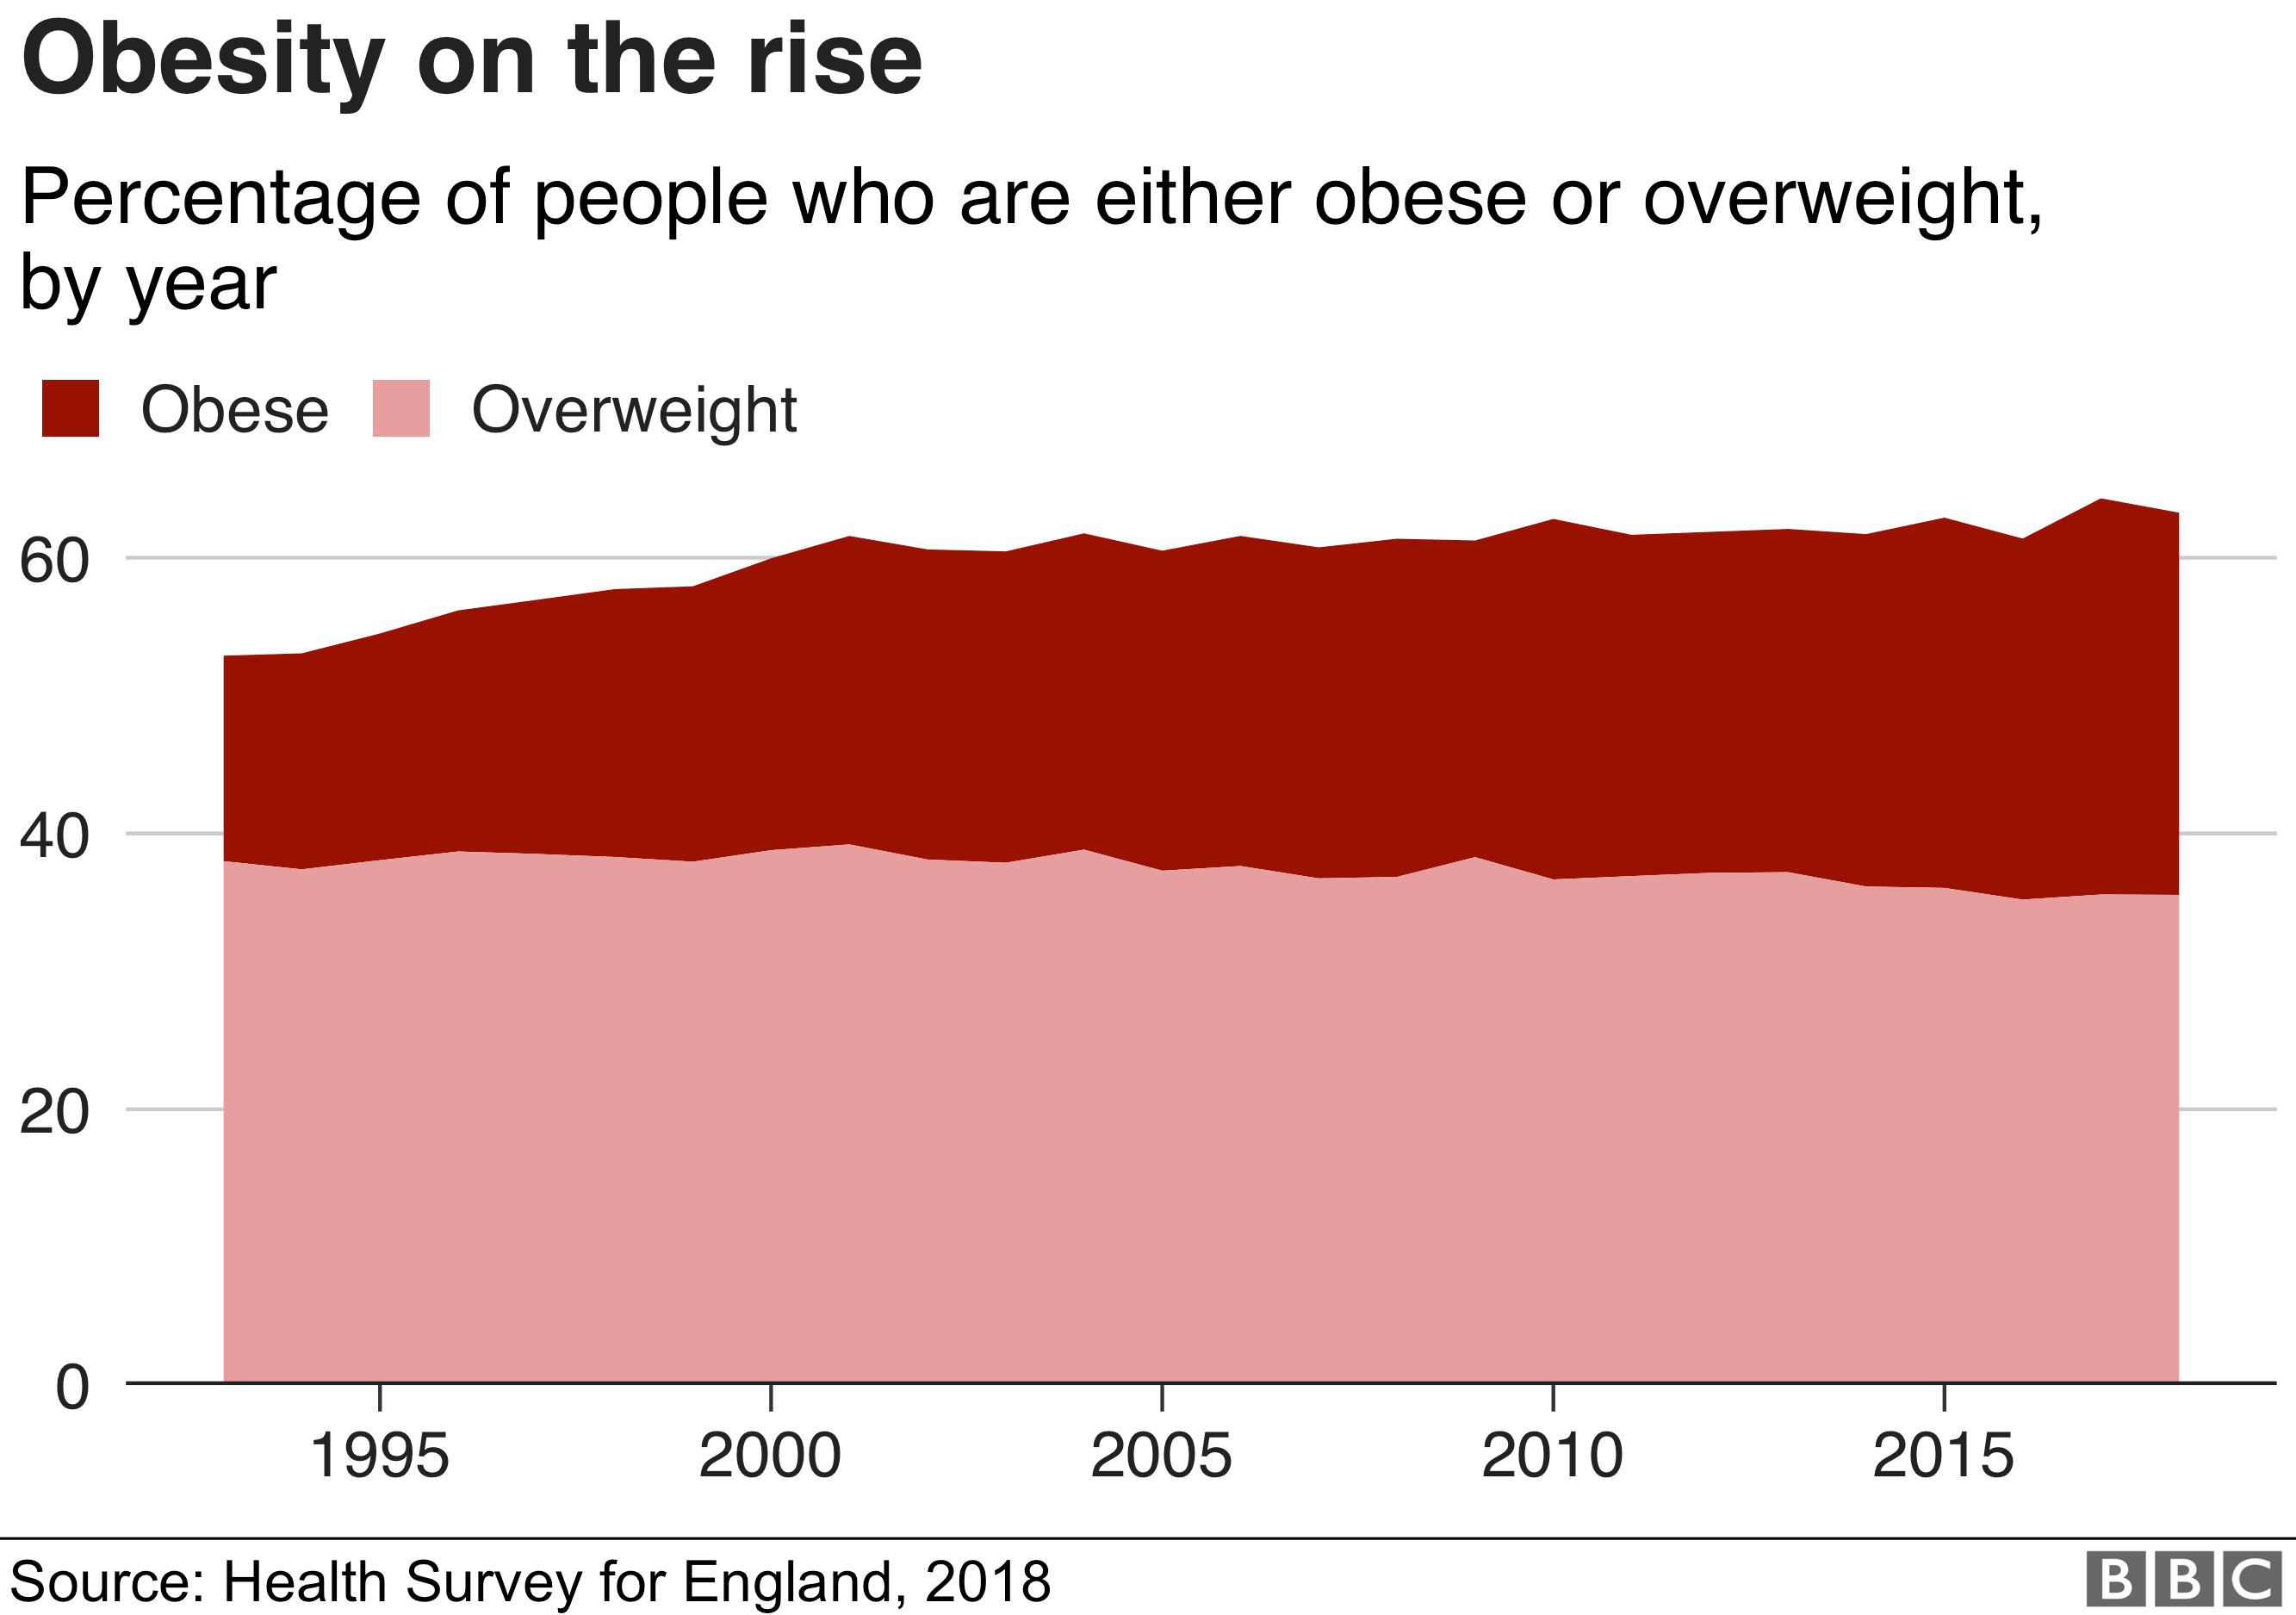
\includegraphics[width=0.67\textwidth]{figures/obesity.png}
        \caption{Percentage of people who are either obese or overweight, by year (Source: Health Survey for England, 2018)}\label{fig:obesity}
    \end{figure}

    To help solve that issue, it is important to encourage people to workout, but going to the gym can be daunting, especially when you don't know how to perform exercises properly. Creating an AI personal trainer will give people the knowledge and confidence to exercise more at home or the gym. Furthermore, exercise has many benefits other than weight loss, it reduces the risk of the issues mentioned above and has been shown to improve mental health \parencite{NHS-benefits}.\\
    

\section{Problem Statement}
    It is difficult to obtain real-time, individualised input for physical exercise, especially when it is done remotely. Exercise enhances both mental and physical health, but without the right supervision, people run the danger of getting hurt and don't obtain the full benefits of working out. The necessity for remote training solutions has been made evident by the COVID-19 outbreak increasing the popularity of working out at home instead of at the gym. Accurate, real-time feedback can be given by a computer-vision based training coach, which can enhance training, reduce the risk of injury, and promote mental health.

    
\section{Scope of the Project} 
    This project aims to create a program that will act as a personal trainer and that will track the mood of the user to determine the effect of physical exercise on acute mood. This means using a computer vision human pose estimator to find the landmarks on the user's body to determine their shape while asking them about their mood before and after an exercise session. This project will not use any deep learning methods to train any models for the recommendation system and repetition counter as no exercise data will be collect due to time constraints. Simple mathematical methods will be applied instead. The only data that will be collected will be user feedback solely for the purpose of evaluating the performance of the program.
    
\section{Structure of the Thesis}
    The structure of the thesis will proceed as follows. First I will perform a literature review of related work about the different uses of Computer Vision methods, this will include reviewing object detection, object segmentation, human pose estimation, and motion capture. I will also quickly review papers that explore the link between physical exercise and its effect on mood and mental health.\\
    Based on the findings from the literature review, I will lay out my aims and objectives for this project with the goal of having them be novel and have little previous research. These aims and objectives will be Specific, Measurable, Assignable, Realistic and Time-related as per the SMART principles.\\
    Following that, I will describe the methodology of the project, outlining the research design, the architecture of the system, the selection of the algorithm, the development environment including the tools and software used and the version control, the ethical considerations of the project, and an analysis of the risks that will potentially be faced.\\
    Subsequently, I will detail how I implemented the program, first by specifying the system requirements (both software and hardware), then I'll move on to recounting of the creation of the application by describing the integration of the model and the real-time processing.\\
    After the creation of the application, this is the creation of the Graphical User Interface (GUI) going through the development of both the frontend and the backend.\\
    The final section necessary for the detailing of the implementation is the testing and debugging with unit testing and integration testing.\\
    For the penultimate chapter, I will evaluate the performance in results and discussion. In this chapter, I will compare this project with existing solution, I will ponder the user feedback from the usability testing, I will go over the limitations of this project, and finally, provide my interpretation of the results.\\
    And Finally, to conclude, I will summarise the findings, describe the contributions to the field, explain the practical implications, make recommendations for future work, and provide my final thoughts on the entire project.
 
% Literature review
\chapter{Literature Review}
% The literature review is an essential requirement of any academic project. A comprehensive review of the literature will provide background to the project and should be used to inform and guide the research to be undertaken for your project, as well as help guide any software solution. It also establishes that what you have done is the result of academic study, rather than an unfounded whim. This section can build upon the literature you investigated in assessment 1 for the proposal document. You should use the feedback from your supervisor to improve upon the final version. 

% It may be helpful to break up this chapter into sections, with each focused on a different topic or aspect of the project.

%This should be a coherent, critical evaluation of relevant academic literature with clear linkage to your project. You may use and build upon the brief literature survey from your project proposal (which you must reference). You should be aiming to produce a literature review that clearly identifies the area of interest your project sits in, and how it aligns with/builds upon the published work. The project aims and objectives should also be revisited here in its own sub-section.

% goal ~4.5k words
% actual 4147 words

% setup the literature review with a short intro on what computer vision and its subfields are

Computer Vision is a subfield of Artificial Intelligence that has for goal to give machines the sense of vision, or in other words, the ability to perceive and recognise objects. Within Computer Vision there are many more subfields, such as object detection, object segmentation, human pose estimation, motion detection, etc. These are the methods I will be looking at in this review.

\section{Object Detection}
    The ability to identify and locate objects in an image or video is one of the fundamental objectives of computer vision. To improve the accuracy and efficiency of object detection, many methods have been developed over time. Histogram of gradients (HOG) and Haar cascades are examples of conventional methods. The Haar cascades, developed by Paul Viola and Michael Jones, use a series of fundamental classifiers to identify objects based on features such as edges and lines that are derived from integral images. Their capacity to recognise faces has earned them particular notoriety \citep{viola2001rapid}. HOG descriptors, which are helpful for recognising pedestrians and other things with different forms, were developed by Navneet Dalal and Bill Triggs. They function by first dividing an image into small cells, then calculating the gradient orientation histogram for each of those cells, and finally normalising the output \citep{dalal2005histograms}.\\

    \begin{figure}[htbp]
        \centering
        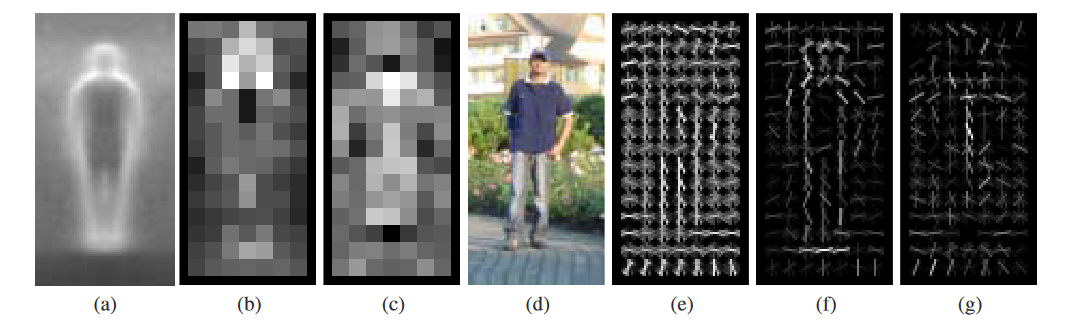
\includegraphics[width=0.99\textwidth]{figures/HOG.png}
        \caption{Navneet Dalal and Bill Triggs' HOG detectors cue mainly on silhouette contours (especially the head, shoulders and feet). The most active blocks are centred on the image background just outside the contour. (a) The average gradient image over the training examples. (b) Each “pixel” shows the maximum positive SVM weight in the block centred on the pixel. (c) Likewise for the negative SVM weights. (d) A test image. (e) It’s computed R-HOG descriptor. (f,g) The R-HOG descriptor weighted by respectively the positive and the negative SVM weights. \citep{dalal2005histograms}}
        \label{fig:HOG}
    \end{figure}

    Deep learning algorithms have considerably improved the detection of objects. Region-Based Convolutional Neural Networks, or R-CNN, by Ross Girshick et al., resorted to a two-step process of generating region proposals and classifying each proposal using a CNN. While this gave better accuracy in detection, it added a large computational cost \citep{girshick2014rich}. Fast R-CNN by Ross Girshick does this with even better performance by integrating the recommendation of regions and classification into a single network. There will be one RoI pooling layer to pool the features of each proposal \citep{girshick2015fast}. Faster R-CNN by Shaoqing Ren et al. incorporates region proposal networks, or RPNs for short, that share some convolutional layers with the detection network to provide near cost-free region proposals, thus speeding up the detection \citep{ren2015faster}. \\

    \begin{figure}[htbp]
        \centering
        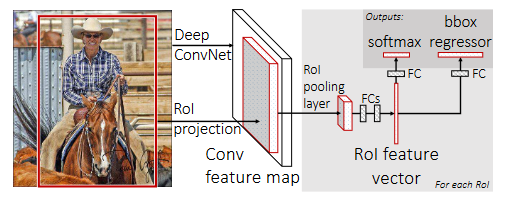
\includegraphics[width=0.80\textwidth]{figures/Fast_R-CNN.png}
        \caption{Fast R-CNN architecture.\citep{girshick2015fast}}
        \label{fig:FastRCNN}
    \end{figure}

    Single Shot MultiBox Detector (SSD) by Wei Liu et al. bypass region proposal completely and use a single network to predict object classes and bounding boxes directly from feature maps at all scales. It goes in direct balance with speed and accuracy for the real-time application \citep{liu2016ssd}. Along this line, Tsung-Yi Lin et al. form the above class imbalance problem in the dense object detection task to the newly introduced function Focal Loss in RetinaNet. This is done by down-weighting the loss of the well-explained model instances to give the most focus to the hard-to-classify instances \citep{lin2017focal}.\\
    
    These methods present the evolution of object detection techniques from traditional ones, based on handcrafted features, to the modern deep learning-based framework with the power of Convolutional Neural Networks. This particular feature is strong in one visual function or another, and choice in using a method can often come down to the specifics of the application requirements, such as speed, accuracy, and computational resources.

\section{Methods of Segmentation}
    Image segmentation is considered one of the most prominent tasks done in the field of computer vision. The process can be defined as partitioning a given image into a number of segments or regions, where every part represents some meaningful portion of the original image. Several schemes have been developed through the years to achieve perfect and efficient segmentation. The classical ones include thresholding, edge detection, and region-based segmentation. Thresholding: This type of simple segmentation simply takes a greyscale image and the threshold values to convert the image into a binary image. All pixels that have intensity values larger than the threshold are considered as foreground, and those with lower intensity values are classified under background. The technique of this kind basically works for those images that have huge differences in the values of intensity between objects and their background \citep{otsu1975threshold}. Edge detection methods, exemplified by the classic one—Canny edge detector—are designed to identify object boundaries in an image by the detection of intensity discontinuities. They are used in applications where it can segment objects having well-defined edges. One of the most used was that developed by John Canny, known as the Canny edge detector, for its ability to detect edges with low error rates and good localisation \citep{canny1986computational}. Methods for region-based image segmentation group pixels together with certain similar properties. The major methods are region growing and region splitting and merging. Region growing does the segmentation from user-specified starting points by picking neighboring pixels that meet the specified criteria. Region splitting and merging divide an image into local regions and then combine them into groups using measures of similarity \citep{adams1994seeded}.\\

    \begin{figure}[htbp]
        \centering
        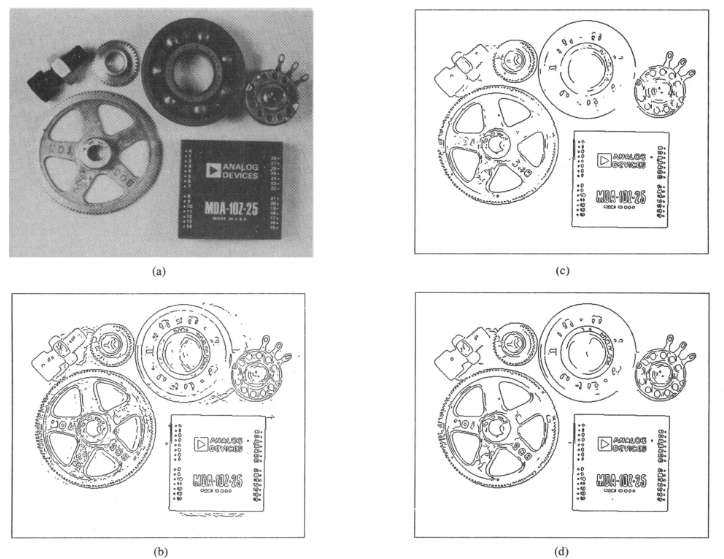
\includegraphics[width=0.49\textwidth]{figures/canny.png}
        \caption{(a) Parts image, 576 by 454 pixels. (b) Image thesholded at T,. (c) Image thresholded at 2 T,. (d) Image thresholded with hysteresis using both the thresholds in (a) and (b). \citep{canny1986computational}}
        \label{fig:canny}
    \end{figure}

    Deep learning techniques have significantly enhanced image segmentation procedures. Fully Convolutional Networks are one kind of neural network designed explicitly for pixel-wise prediction tasks by Jonathan Long et al. In general, an FCN is an extension of the traditional CNNs; it replaces fully connected layers with convolutional layers so that the network outputs a segmentation map of the same size as the input image. It increased the accuracy of semantic segmentation to a large extent \citep{long2015fully}. Probably the most popular biomedical image segmentation architecture is the U-Net introduced by Olaf Ronneberger et al. The U-Net represents a network with an encoder-decoder architecture that provides high-resolution features from the encoder, which are concatenated with upsampled features from the decoder through skip connections. This design enables retaining spatial information and improves segmentation accuracy \citep{ronneberger2015u}. Mask R-CNN, introduced by Kaiming He et al., extends Faster R-CNN with an added branch for predicting a segmentation mask on each Region of Interest (RoI). While Faster R-CNN just localises the object, the method can do instance segmentation—in that each object instance is segmented on its part. Widespread adoption has taken place due to the accuracy and versatility of Mask R-CNN \citep{he2017mask}. The DeepLab was developed by Liang-Chieh Chen et al. and uses atrous or dilated convolutions to stride contextual information at multiple scales without losing resolution. DeepLab also integrates Conditional Random Fields that help refine segmentation borders, enabling it to effectively segment complex-shaped and scale-varying objects \citep{chen2017deeplab}.\\

    \begin{figure}[htbp]
        \centering
        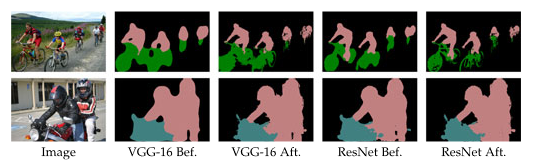
\includegraphics[width=0.99\textwidth]{figures/deeplab.png}
        \caption{DeepLab results based on VGG-16 net or ResNet-101 before and after CRF. The CRF is critical for accurate prediction along object boundaries with VGG-16, whereas ResNet-101 has acceptable performance even before CRF.\citep{chen2017deeplab}}
        \label{fig:deeplab}
    \end{figure}

    The methods include traditional heuristic approaches to image segmentation and more advanced and deep learning-based frameworks that are empowered by neural networks. Each of the methods will have a share in strong and weak points and be more suitable for certain applications than others depending on the accuracy required, computational efficiency, and the type of complexity involved in the segmentation.
    

\section{Human Pose Estimation (HPE)}
    Human pose estimation is a process for detecting and tracking the location of key body joints in images or videos; it is thus of paramount importance in the field of computer vision. This has been applied to motion capture, activity recognition, human–computer interaction, and other areas. Two traditional solutions are pictorial structures and deformable part models. Pictorial structures model a human body as a collection of rigid parts connected by flexible joints. Each part is modeled using a template, and configuration of parts is optimised to fit the observed image. This framework, thanks to Felzenszwalb and Huttenlocher has been quite successful in detecting human poses in static images \citep{felzenszwalb2005pictorial}. Deformable Part Models generalise pictorial structures to allow for deformation of parts relative to each other. Felzenszwalb et al.'s method represents the object class by a mixture of templates, each capturing appearance and pose variations. DPMs have been used in many applications involving object detection and human pose estimation \citep{felzenszwalb2009object}.\\

    \begin{figure}[htbp]
        \centering
        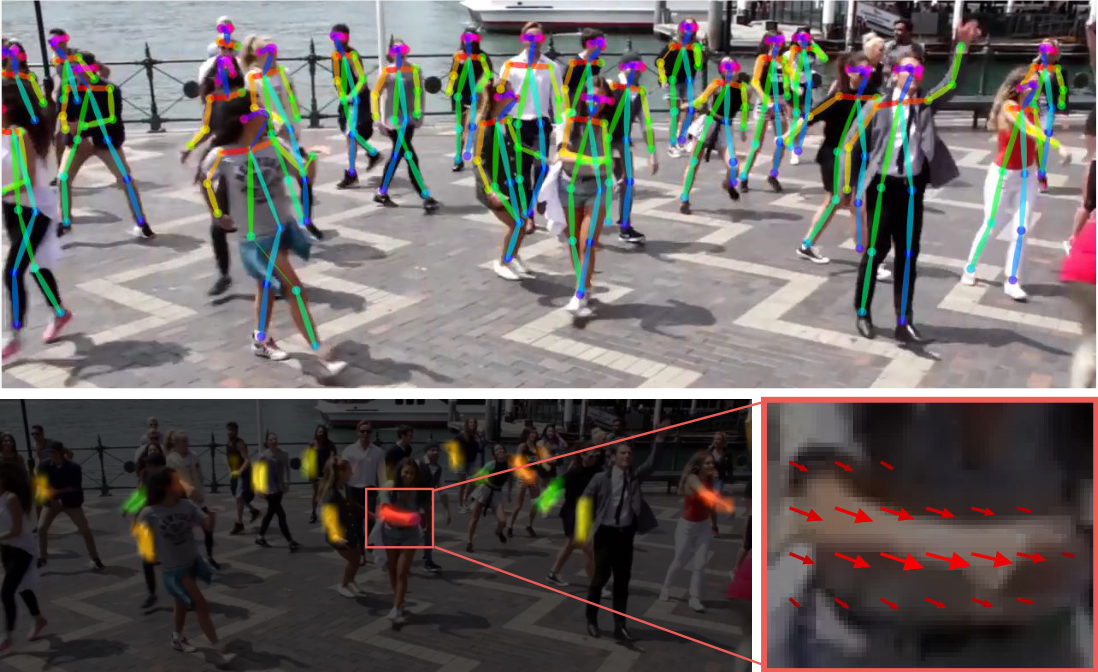
\includegraphics[width=0.49\textwidth]{figures/multipose.png}
        \caption{Top: Multi-person pose estimation. Body parts belonging to the same person are linked. Bottom left: Part Affinity Fields (PAFs) corresponding to the limb connecting right elbow and right wrist. The color encodes orientation. Bottom right: A zoomed in view of the predicted PAFs. At each pixel in the field, a 2D vector encodes the position and orientation of the limbs. \citep{cao2017realtime}}
        \label{fig:multipose}
    \end{figure}

    Deep learning-based methods have greatly advanced human pose estimation. Employing a sequence of convolutional networks to iteratively predict the locations of body joints, the Convolutional Pose Machines method has already shown very accurate results. In each stage of this network, it is expected to refine the prediction in the previous stage, hence improving the accuracy in pose estimation iteratively \citep{wei2016convolutional}. The Stacked Hourglass Networks by Newell et al. uses symmetric encoder-decoder architecture capturing features at many scales. Such a network is made up of many hourglass modules stacked together, so that it is feasible to perform bottom-up and top-down processing repetitively. This algorithmic approach has achieved a top performance in human pose estimation \citep{newell2016stacked}. OpenPose, developed by Cao et al., is a real-time multi-person pose estimation framework. It uses a two-branch CNN to predict part affinity fields (PAFs) and keypoint locations simultaneously. PAFs encode the spatial relationships between body parts, enabling the network to associate detected keypoints with individual people in the image \citep{cao2017realtime}. PoseNet by Kendall et al. comprises a deep learning framework for estimating human poses from images. This approach uses a CNN to directly predict the 2D coordinates of body joints from an input image and can be end-to-end trained to solve a wide variety of pose estimation tasks. PoseNet has been identified to work quite well in terms of accuracy and to be very robust in very challenging conditions \citep{kendall2015posenet}.\\

    \begin{figure}[htbp]
        \centering
        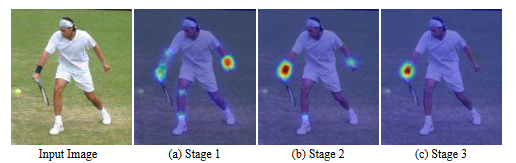
\includegraphics[width=0.75\textwidth]{figures/convPose.png}
        \caption{Here Wei et al. show the increasingly refined estimates for the location of the right elbow in each stage of the sequence. (a) Predicting from local evidence often causes confusion. (b) Multi-part context helps resolve ambiguity. (c) Additional iterations help converge to a certain solution. \citep{wei2016convolutional}}
        \label{fig:convpose}
    \end{figure}
    
    These methods reflect the journey that began with traditional approaches, which relied on handcrafted models for human-pose estimation, to deep-learning-based advanced frameworks exploiting the power of convolutional neural networks. Each approach has its strengths and weaknesses, and very often, the choice of method depends on the kind of application at hand, that is, accuracy, computational efficiency, or the complexity of poses estimated.
    

\section{Motion Tracking}
    One of the big modules of computer vision, motion tracking involves the tracking of a human or any other entity from one frame to another in a video sequence. Major applications include surveillance, sports analysis, and augmented reality. Traditional approaches include optical flow, the Kalman filter, and mean shift. Most of the approaches in use for calculating the motion of an object via optical flow generally make use of the apparent motion of the brightness patterns between consecutive frames. Probably the most famous among these, which assumes constant flow in some small neighbourhood and finds the motion using least squares fitting, is the method proposed by Bruce D. Lucas and Takeo Kanade \citep{lucas1981iterative}. Another popular method is based on the Horn-Schunck algorithm with the smoothness constraint of the flow field in order to cope with noise and discontinuities \citep{chen2016full}. Basically, the Kalman filter is a principle of state estimation for a dynamic system from noisy observations by a recursive algorithm. Since it finds applications in prediction regarding position and velocity for moving objects, it is normally used in motion tracking. Prediction and update are basically the two working steps of the Kalman filter, and the same have been designed efficiently to handle problems regarding real-time tracking \citep{kalman1960new}. Mean shift is a non-parametric feature-space analysis technique applied for finding the maxima of a density function. Applied to motion tracking, it shifts a window iteratively to the area with the highest density of features and uses it to track an object. Thus, this approach is robust against appearance variations of the object and partial occlusions \citep{comaniciu2000real}.\\

    \begin{figure}[htbp]
        \centering
        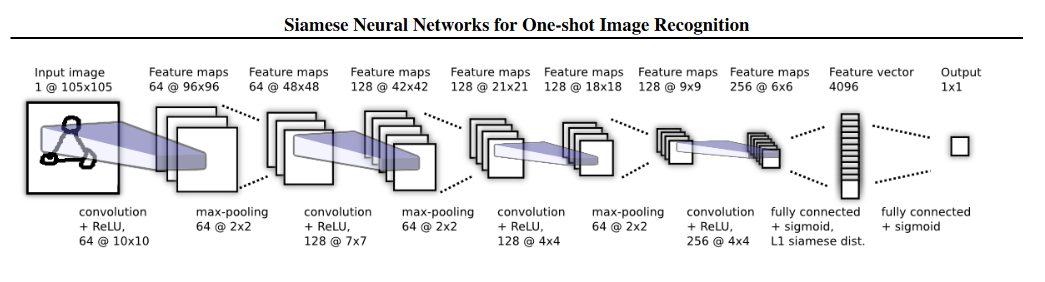
\includegraphics[width=0.99\textwidth]{figures/siamese.png}
        \caption{Best convolutional architecture selected for verification task. Siamese twin is not depicted, but joins immediately after the 4096 unit fully-connected layer where the L1 component-wise distance between vectors is computed \citep{koch2015siamese}}
        \label{fig:siamese}
    \end{figure}

    Deep learning methods have already shown a high improvement in the state-of-the-art performance in motion tracking. RNNs, and especially the LSTM network, conduct motion tracking through modelling temporal dependencies in sequential data. They hence learn how to predict the future positions of objects from their previous trajectories and hence can be applied to track complicated nonlinear motions \citep{hochreiter1997long}. Koch et al. have proposed Siamese networks for application in one-shot learning problems like object tracking. It consists of two identical sub-networks processing two different inputs and returning the similarity score as output. In the case of motion tracking, the Siamese Networks could be trained for the differentiation of target from background and offer robustness under challenging conditions \citep{koch2015siamese}. DeepSORT hybridises the SORT algorithm with a deep appearance descriptor. This approach uses a CNN for extracting features from detected objects and a Kalman filter, which provides motion prediction. By combining both appearance and motion information, this significantly improves not only accuracy but also resilience in tracking \citep{wojke2017simple}. Huang et al. proposed a deep framework called TrackNet for sports tracking. It uses a CNN to predict the heatmap in every frame on the location of the target and further refines these predictions with post-processing. On the other hand, TrackNet was able to track fast-moving targets such as the badminton shuttlecock and tennis ball \citep{huang2019tracknet}. \\

    \begin{figure}[htbp]
        \centering
        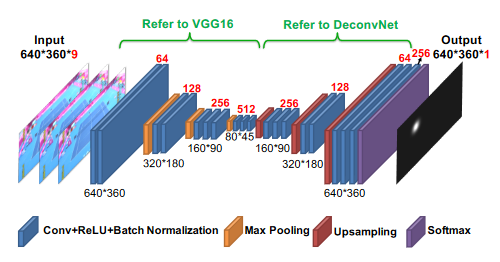
\includegraphics[width=0.6\textwidth]{figures/tracknet.png}
        \caption{The architecture of the proposed TrackNet \citep{huang2019tracknet}}
        \label{fig:tracknet}
    \end{figure}

    These methods very clearly show how far the progress of motion-tracking techniques has moved from more traditional, math-model-based methods to advanced, deep learning-based frameworks that exploit the power of neural networks. But each has its strengths and weaknesses, and often, the choice of the method depends on the specific requirements of the application.

\section{The Cutting Edge of HPE}
    There has been huge progress in HPE, with sophisticated models like YOLO  by Ultralytics and Google's MediaPipe. While both of these frameworks offer very powerful detection and tracking tools for human pose, they differ in approach and capabilities. 
    \begin{figure}[htbp]
        \centering
        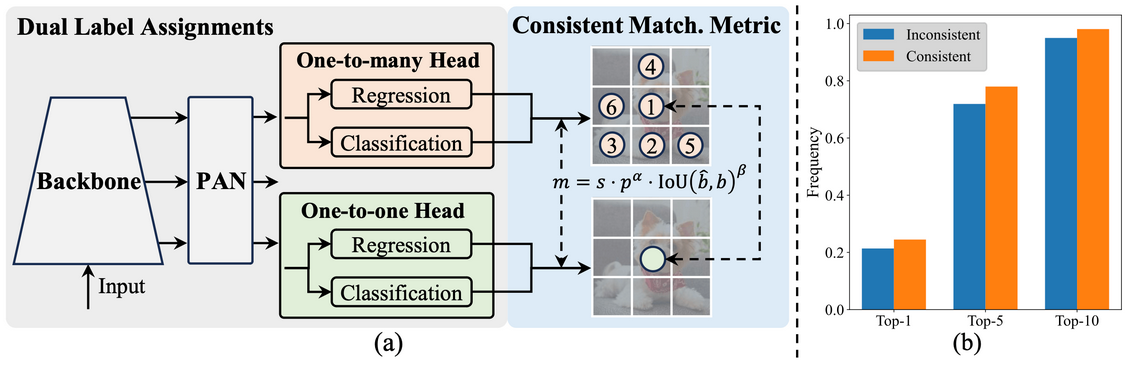
\includegraphics[width=0.8\textwidth]{figures/yolov10arch.png}
        \caption{(a) Consistent dual adddignments for NMS-free training. (b) Frequency of one-to-one assignments in Top-1/5/10 of one-to-many results for YOLOv8-S which employs $\alpha_{o2m}$=0.5 and $\beta_{o2m}$=6 by default. (https://docs.ultralytics.com/models/yolov10/)}
        \label{fig:yolo_arch}
    \end{figure}
    \subsection{YOLO by Ultralytics}
        YOLO stands for 'You Only Look Once,' referring to a family of real-time object detection models that have evolved significantly since their appearance. The newest version, YOLOv10, will raise the power from its predecessors to even more performance and versatility. Joseph Redmon et al. developed the first model for YOLO. It introduced a single unified architecture processing full images in pass-through, very fast \citep{redmon2016you}. Batch Normalisation, Anchor Boxes, and Dimension Clusters improve YOLOv2 \citep{redmon2017yolo9000}. It was succeeded by YOLOv3, which again pushed model performance by an enhanced and more lightweight backbone network with multiple anchors \citep{redmon2018yolov3}. Then, mosaic data augmentation and a new anchor-free detection head were introduced in YOLOv4 \citep{bochkovskiy2020yolov4}. Then, YOLOv5 from Ultralytics had a couple of interesting features, one of which was hyperparameter optimisation with integrated experiment tracking \citep{jocher2020yolov5}. Thereafter, Li et al. published YOLOv6, which was optimised for autonomous delivery robots \citep{li2022yolov6}. More enhancements were added to YOLOv7, and extra tasks like human pose estimation on COCO keypoints \citep{wang2023yolov7}. YOLOv8 is a highly versatile and efficient approach, ranging from detection to segmentation with human pose estimation and tracking, and classification \citep{ultralytics2023yolov8}. Later, YOLOv9 proposed the new programmable gradient information concept along with a new lightweight network architecture, GELAN, to further hugely improve the use of parameters and performance on MS COCO \citep{wang2024yolov9}. Finally, to this end, YOLOv10 went ahead in efficiency by innovating consistent dual assignments for NMS-free training, with holistic efficiency-accuracy-driven model design strategies to achieve SOTA performance and efficiency across various model scales \citep{wang2024yolov10}.

        \begin{figure}[htbp]
            \centering
            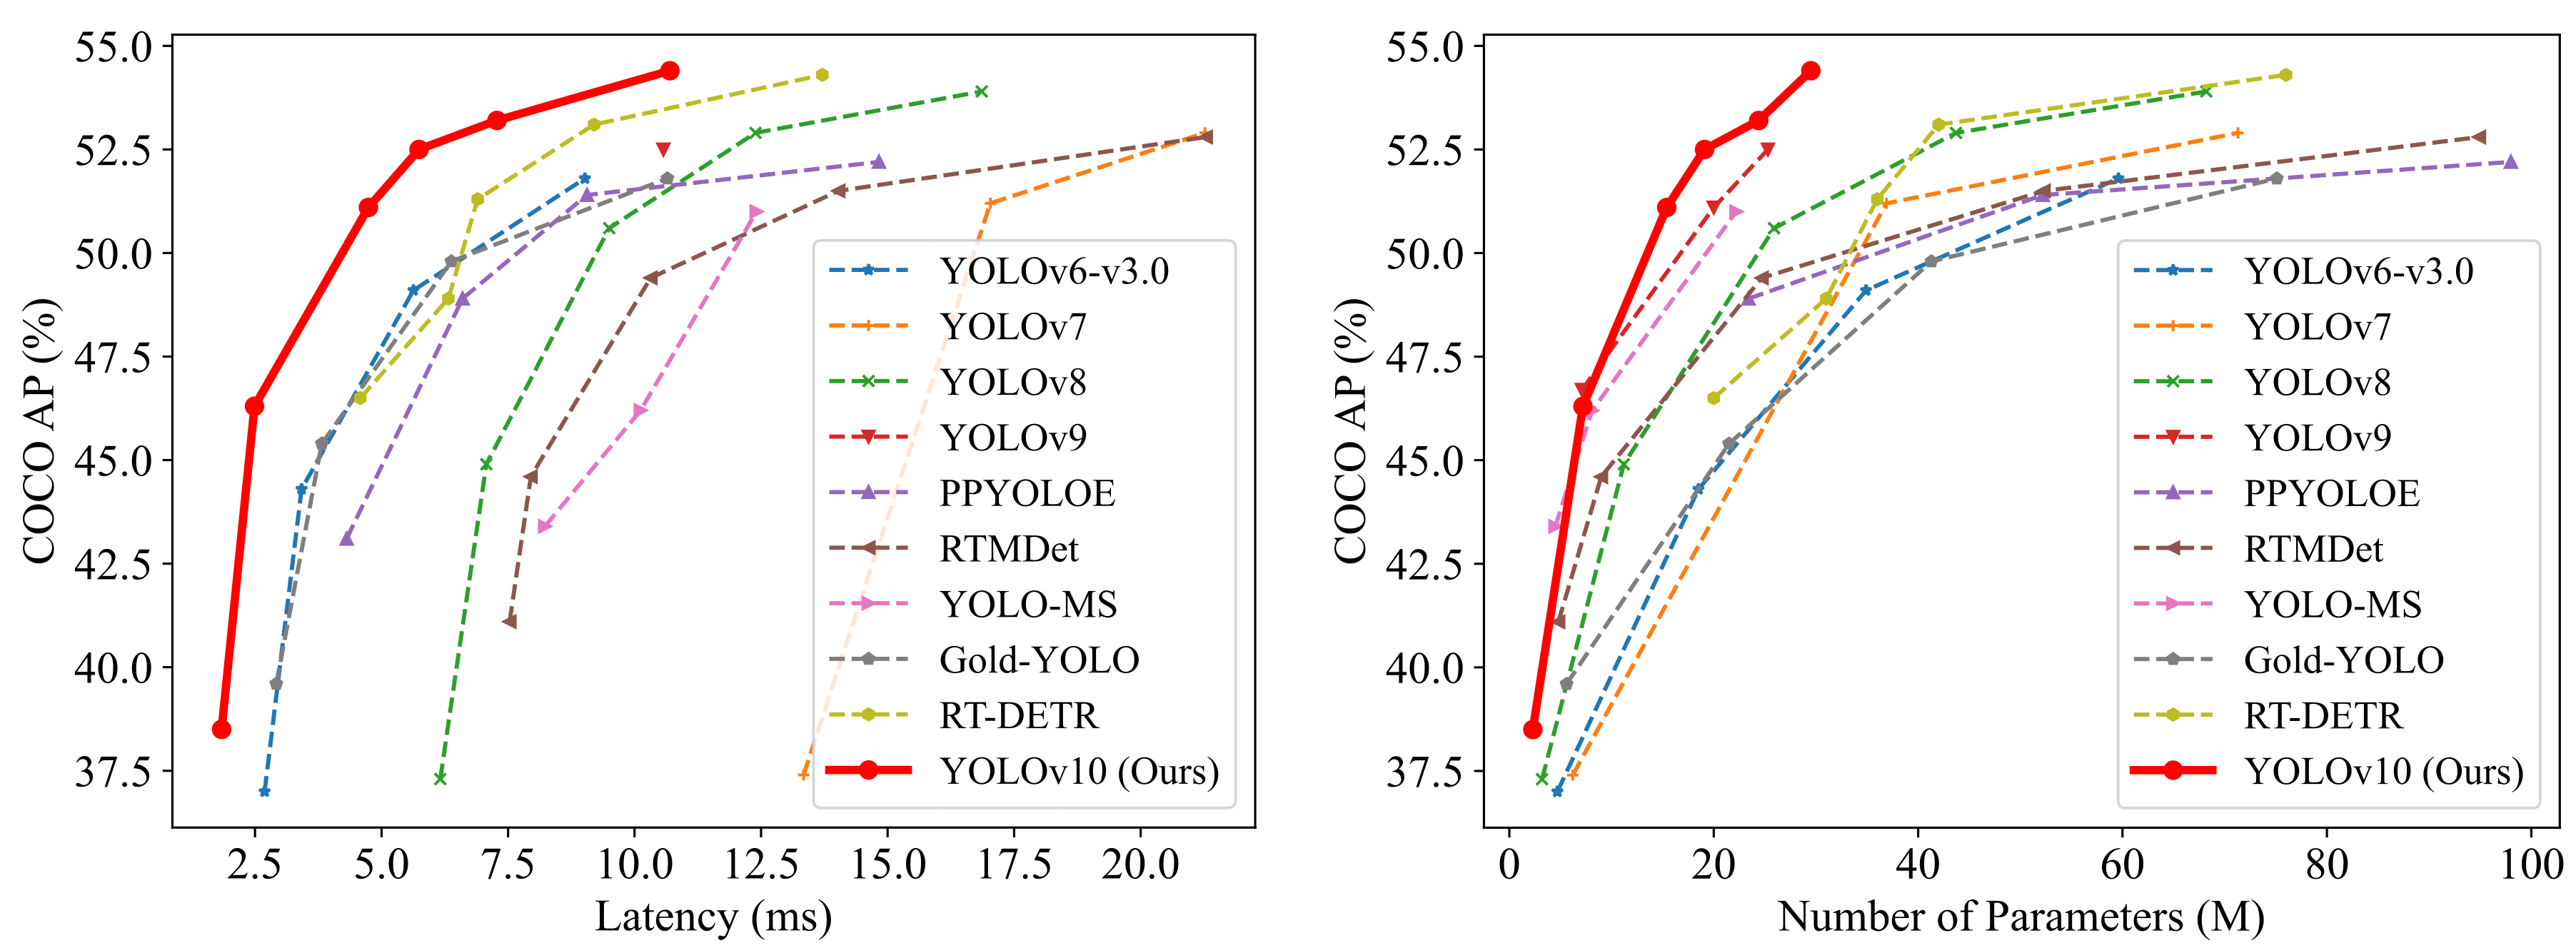
\includegraphics[width=0.8\textwidth]{figures/yolov10comp.png}
            \caption{Comparision of various models including the YOLO models v6 to v10 (https://docs.ultralytics.com/models/yolov10/)}
            \label{fig:yolo_comp}
        \end{figure}
    \subsection{Mediapipe by Google}
        MediaPipe is an open-source framework developed by Google that enables cross-platform, customisable ML across live and streaming media. It is designed to be highly flexible and to be easily integrated into a range of applications. MediaPipe provides the most complete solution for pose estimation, which is realised through a two-stage detector: first, ROI detection containing the person, then keypoint prediction inside. This methodology assists in accurate estimation of pose in real-time \citep{lugaresi2019mediapipe}. MediaPipe is very flexible; it has developed models and pipelines that can be easily customised for a developer's requirements. It supports a great variety of platforms, including Android, iOS, web, and desktop, hence making it quite accessible for various applications \citep{google2023mediapipe}. MediaPipe has been used in a host of different applications, from fitness tracking to augmented reality. On the other hand, it is a popular choice among many developers who want to implement pose estimation and several other computer vision tasks because of the capability to handle a myriad of modalities, like video or audio, and the ease of integration \citep{lugaresi2019mediapipe}. Recent improvements to MediaPipe include hand-gesture recognition by improving the framework for 3D keypoint estimation more accurately and adding support for neural network-based gesture classifiers \citep{sung2021device}.

        \begin{figure}[htbp]
            \centering
            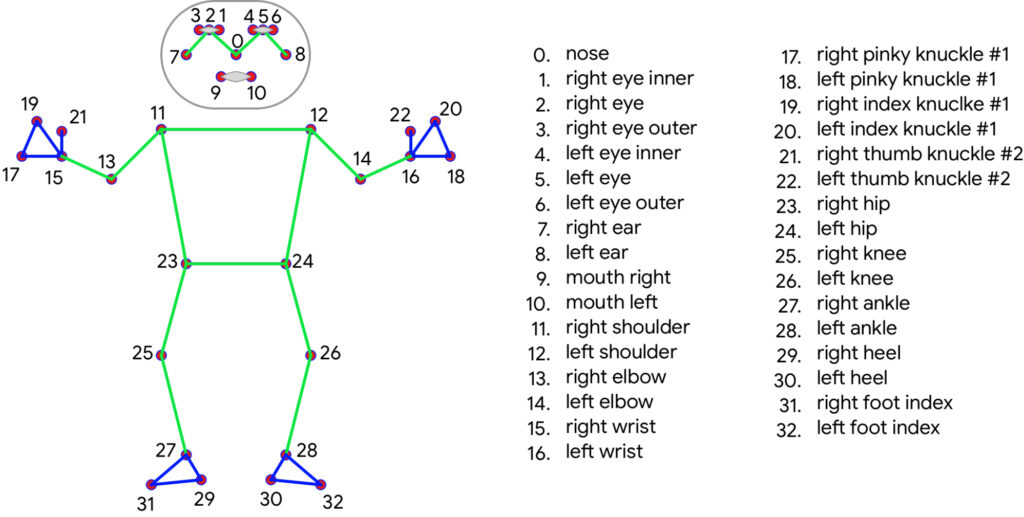
\includegraphics[width=0.75\textwidth]{figures/mediapipe.png}
            \caption{The body keypoints used by mediapipe}
            \label{fig:mediapipe}
        \end{figure}
    \subsection{Comparison}
        Let's compare these two solutions:
        \begin{enumerate}
            \item \textbf{Speed and Performance}\\
            YOLO:
            \begin{itemize}
                \item \textbf{Real-time Processing}: Models in YOLO are very fast and process natural images in real time. This makes them very appropriate to any application including immediate feedback, for example, live video analysis and autonomous systems.
                \item \textbf{Unified Architecture}: YOLO’s single-pass architecture allows it to detect objects and poses in one go, significantly reducing latency compared to multi-stage detectors.
            \end{itemize}
            MediaPipe:
            \begin{itemize}
                \item \textbf{Two-Stage Detection}: MediaPipe uses a two-stage approach: first, it detects the ROI and then predicts keypoints within the ROI. Compared with YOLO's single pass, this is slightly slower but often more accurate for pose estimation.
                \item \textbf{Optimised for Mobile and Web}: MediaPipe is designed to run efficiently on various platforms, including mobile devices and web browsers, ensuring smooth performance even on less powerful hardware.
            \end{itemize}
            \item \textbf{Flexibility and Customisation}\\
            YOLO:
            \begin{itemize}
                \item \textbf{Versatility}: In addition to position estimation, YOLO models—especially the most recent iterations, such as YOLOv8 and YOLOv10—support a variety of tasks, such as object detection, segmentation, and tracking. Because of its adaptability, YOLO is an effective tool for extensive AI vision applications.
                \item \textbf{Customisation}: YOLO allows for extensive customisation through hyperparameter tuning and integration with various frameworks, enabling developers to optimise the model for specific use cases.
            \end{itemize}
            MediaPipe:
            \begin{itemize}
                \item \textbf{Modular Design}: MediaPipe's modular architecture makes pipeline customisation and extensibility very convenient for developers to make precisely whatever application may be needed—be it a fitness tracker or an augmented reality application.
                \item \textbf{Cross-Platform Support}: MediaPipe’s ability to run on Android, iOS, web, and desktop platforms makes it highly adaptable for different deployment environments.
            \end{itemize}
            \item \textbf{Accuracy and Robustness}\\
            YOLO:
            \begin{itemize}
                \item \textbf{High Accuracy}: Accuracies of YOLO models have increased with each successive edition. For example, YOLOv10 introduces state-of-the-art techniques, such as consistent dual assignments and holistic efficiency-accuracy-driven design, to achieve state-of-the-art performance.
                \item \textbf{Robustness}: YOLO’s robust architecture and extensive training on diverse datasets ensure reliable performance across various scenarios, from crowded scenes to low-light conditions.
            \end{itemize}
            MediaPipe:
            \begin{itemize}
                \item \textbf{Precision}: The two-stage strategy of detection is very often accurate in MediaPipe pose estimation; therefore, it's applicable in various domains, from medical diagnosis to sports analysis.
                \item \textbf{Multi-Modal Capabilities}: MediaPipe’s support for multiple modalities (e.g., video, audio) enhances its robustness in handling complex tasks that require integrating different types of data.
            \end{itemize}
            \item \textbf{Ease of Integration}\\
            YOLO:
            \begin{itemize}
                \item \textbf{Integration with AI Frameworks}: YOLO models can be easily integrated with popular AI frameworks like TensorFlow, PyTorch, and ONNX, facilitating seamless deployment in various environments.
                \item \textbf{Community and Support}: The extensive community support and comprehensive documentation available for YOLO models make it easier for developers to implement and troubleshoot.
            \end{itemize}
            MediaPipe:
            \begin{itemize}
                \item \textbf{Ease of Use}: MediaPipe also provides out-of-the-box solutions and configurable pipelines, making integration easy. Also, with its intuitive API and broad reach of documentation, it empowers developers who have minimal experience in computer vision.
                \item \textbf{Google Ecosystem}: As part of the Google ecosystem, MediaPipe benefits from continuous updates and improvements, ensuring compatibility with the latest technologies and platforms.
            \end{itemize}
            \item \textbf{Use Cases}\\
            YOLO:
            \begin{itemize}
                \item \textbf{Real-Time Applications}: Ideal for applications requiring real-time processing, such as autonomous driving, surveillance, and live sports analysis.
                \item \textbf{Comprehensive Vision Tasks}: Suitable for projects that need a versatile model capable of handling multiple vision tasks simultaneously.
            \end{itemize}    
            MediaPipe:
            \begin{itemize}
                \item \textbf{Custom Solutions}: Perfect for applications that require tailored solutions, such as fitness apps, augmented reality, and interactive media.
                \item \textbf{Cross-Platform Deployment}: Best suited for projects that need to run on various platforms, including mobile devices and web browsers.
            \end{itemize}
        \end{enumerate}
        In summary, while both YOLO and MediaPipe provide very powerful tools for tasks in the estimation of human pose, the former comes short in flexibility, ease of integration, and cross-platform support. It is perfect for those applications that require bespoke solutions with seamless deployment across all platforms, thanks to its modular design and capability for handling multiple modalities. Regarding the project in this paper, MediaPipe seems the better choice.

\section{The Effect of Exercise on Mood}
    It has been known for decades that one's mental health can be improved by incorporating exercise into their lifestyle. The papers titled "The relation of physical activity and exercise to mental health." \citep{taylor1985relation} and "Psychological effects of habitual aerobic exercise: A critical review" \citep{hughes1984psychological} were early studies on this phenomenon and to what extent physical activity affects mental health. By reviewing controlled experiments on the effects of habitual aerobic exercise on mood, personality, and cognition, Tayor et al. found that the strongest evidence suggests that exercise will most likely alleviate symptoms of depression, alcoholism, anxiety, and schizophrenia, as well as improve self-image and social skills.\\
    This more recent review titled "Physical exercise and mental health: The routes of a reciprocal relation" \citep{fossati2021physical} looks at the physical-mental link in the other direction, looking to find whether this relationship is reciprocal.\\
    Finally, the study "Effects of a bout of exercise on mood in people with depression with and without physical pain" \citep{caviness2023effects} investigates the immediate effect of aerobic exercise on a community sample of 147 participants with above-average depressive symptoms by recording their mood before and after the activity. They found a statistically significant change between pre and post-workout mood.\\
    The question for this paper is: does this mood change still happen if the exercise is not aerobic, such as resistance training and callisthenics?

\section{Summary}
    Object detection, segmentation, human pose estimation, and motion tracking have all benefited from corresponding development from traditional methods up to modern deep learning frameworks. Classic techniques in the line of HOG, Haar cascades, thresholding, edge detection, and Kalman filters did much to lay the ground. Deep learning has reshaped these with R-CNN, U-Net, Convolutional Pose Machines, and LSTM networks, attaining more accuracy and efficiency. State-of-the-art solutions, such as YOLO and MediaPipe, are real-time, versatile, and cross-platform, really stretching the bounds of what could be done within computer vision.
    \subsection{Comparison of the Current Solutions}
        There are solutions to computer vision problems in terms of speed, accuracy, and suitability of applications. Most of the traditional methods are normally simple, less computationally intensive, and poor in terms of accuracy and robustness against deep approaches. Deep learning methods, like Faster R-CNN for detection and U-Net for segmentation, will rather be at the high end in terms of accuracy but at an expensive computational cost. On the other hand, YOLO models would give a compromise in speed and accuracy that is of relevance in real-time applications. MediaPipe offers flexibility and ease of integration across platforms on the other side.
    \subsection{Research Gaps}    
        While the achievements that have been made so far in this area are very inspiring, there are still some gaps in the research. The first gaps, even though this is an area which is improving, are efficient models that can run on low-power devices without a loss of accuracy. Handling of occlusions and light variation is another challenge that is currently a goal for researchers. Better generalisation across different datasets and environments, and more robust methods for real-time multi-object tracking and pose estimation in crowded scenes, are required. Addressing these gaps will be highly instrumental in taking further applications of computer vision forward.

\section{Aims \& Objectives}

% Having situated your project within a body of relevant literature, you should now be in a position to state your aims and objectives. These should be broadly similar to those given in your proposal. Most projects will have one aim that is a broad statement of what the project will achieve. The objectives should be statements of how that aim will be achieved. Objectives should be Specific, Measurable, Assignable, Realistic and Time-related (SMART).
    Based on the previous research described in the literature review above, I can know express my aims and objectives for this project. Here are the SMART goals I have set for this endeavor:

    \begin{enumerate}
        \item \textbf{Specific}: The goal of creating an AI fitness trainer application that will set the groundwork for studying the effect of exercise on mood. It involves these tasks:
        \begin{itemize}
            \item \textbf{User Detection}: Using video input to detect the presence of the user ensures the application can start analysing only when a user is present.
            \item \textbf{Keypoint Identification}: Identifying keypoints on the user's body is crucial for understanding body posture and movement.
            \item \textbf{Pose Analysis}: Analysing the poses created by the connections between keypoints allows the application to understand the user's form and make necessary inferences about occluded keypoints.
            \item \textbf{Form Recommendations}: Providing recommendations to improve the user's form help in minimising injury risks and maximising exercise effectiveness.
            \item \textbf{Mood Tracking}: Collecting the mood of the user before and after the exercise session.
            \item \textbf{Potential Add-on}: Developing a smartphone application enhances accessibility and user convenience.
        \end{itemize}
        
        \item \textbf{Measurable}: The success of the application can be qualitatively measured through:
        \begin{itemize}
            \item \textbf{Detection Accuracy}: The ability to accurately detect the human shape and keypoints. This is quantitatively measurable through metrics such as balanced accuracy, f1 score, precision, recall...
            \item \textbf{User Feedback}: Collecting user feedback on the effectiveness of the recommendations provided by the application. This is a more qualitative measure as the users' feedback will take the form of reviews. The users can be asked to give scores for usability and perceived effectivness.
        \end{itemize}
        
        \item \textbf{Achievable}: This project is achievable due to several factors:
        \begin{itemize}
            \item \textbf{Experience}: I have previous experience with image processing using Python providing a solid foundation for developing this application. As during my MComp degree, I worked on a project that detected and tracked seabirds on timelapse images using YOLOv5, tracking the birds from egg to adult stage. 
            \item \textbf{Existing Technologies}: By leveraging existing libraries and frameworks for computer vision (e.g. OpenCV, MediaPipe) can accelerate development.
            \item \textbf{Incremental Development}: By breaking down the project into smaller, manageable tasks ensures a steady progress and allows for iterative improvements.
        \end{itemize}
        
        \item \textbf{Relevant}: The project is highly relevant for several reasons:
        \begin{itemize}
            \item \textbf{Health and Fitness}: With the growing emphasis on physical and mental health and fitness, an AI personal trainer can provide valuable assistance to users looking to improve their exercise routines.
            \item \textbf{Injury Prevention}: Proper form is crucial in preventing injuries during exercise, and this application can play a significant role in educating users.
            \item \textbf{Technological Advancement}: This project contributes to advancements in AI and computer vision, showcasing practical applications of these technologies. This also creates a framework on which future research on the effect exercise as on mental health.
        \end{itemize}
        
        \item \textbf{Timebound}: The project has a clear deadline of August 29th, 2024, providing a two-month timeframe. This is sufficient for:
        \begin{itemize}
            \item \textbf{Initial Development}: Completing the core functionalities of user detection, keypoint identification, and pose analysis.
            \item \textbf{Testing and Refinement}: Conducting thorough testing and refining the application based on feedback.
        \end{itemize}
        
    \end{enumerate}  


% Requirements analysis
\chapter{Methodology}
% Drawing upon the research you've conducted; this goal of this chapter is to select and rationalise the research and/or software methods required to meet your project objectives. For example, the choice of quantitative or qualitative methods and the types of statistical or other analysis methods. You should also include software methodologies that are relevant to any development work required to support the project’s research.

% This section will vary greatly depending on your project, and may include sections on topics including (but not limited to) project management, software development methodology, algorithm/model choices, study design, research methods, statistical analysis, performance evaluation, etc. As such, you should discuss the most appropriate approach for developing this section with your supervisor. As this is a Masters-level research project, you must also include a critical discussion on the selected quantitative or qualitative research methods adopted for the project work.

% goal ~2.5k words
% actual 2483 words

\section{Research Design}
    %Outline the overall strategy and framework that guided the research. Include the rationale for choosing specific methods and how they align with the objectives.
    The design of the project follows a qualitative research approach that focuses majorly on user feedback as a way to assess whether or not the effectiveness of the computer-vision-based training coach is at its best. This was done so as to derive specific information touching on the user experience and satisfaction derived from the system by its users.
    \subsection{Qualitative Methods}
        The qualitative methods provided subjective data regarding the user's experience and satisfaction. In this case, the system users were subjected to a semi-structured interview so as to gather feedback on usability, intuitiveness, and overall user experience, The data was important in the identification of weak point and thus assuring the usability and meeting of the needs expected of the system.
    \subsection{Interviews}
        It included semi-structured, in-depth interviews taken with a set of subjects, both novice and experienced users, On its part, it allowed for open-ended responses and gave rich qualitative data about the experiences of the participants.
    \subsection{Rational for Qualitative Approach}
        The qualitative approach was chosen for eliciting in-depth understanding of the user experience. This could be done quantitatively, which would probably be more objective in regard to data about performance of the system, but it would miss fine details about user satisfaction and usability. Interviews were used to gather qualitative data that contributed useful information for the improvement of the system.
    \subsection{Algorithm Validation}
        While the focus of this study is on qualitative assessment, it should not go unmentioned that many research studies have already been done regarding the quantitative testing and validation of the Mediapipe algorithm used for human pose detection. This has established the ground for the accuracy and reliability of the algorithm previously to work in different contexts, thus forming a basis for application in this project. This allows for focusing on a review of the user experience, leaving out the technical accuracy matters at the core because of the use of an algorithm with a good performance history.
\section{System Architecture}
    %Descruve the overall architecture of the system developed for the study. Include the components of the system, their interactions, and how they contribute to achieving the objectives.
    Basically, the system architecture of the computer-vision based training coach has three parts: the applications, the GUI, and the database. The modules are very key to attaining the objectives of the study, for they play a role in the correct detection of human pose, user-friendly interaction, and efficiency in managing data.
    \subsection{Applications}
        The applications incorporate core system functionality, human pose detection, and infer relevant information like joint angles and repetition counts. Each exercise type (e.g. bicep curls) has its own application script. This component is implemented using advanced computer vision algorithms and machine learning models.
        \subsubsection{Human Pose Detection}
            Keypoint detection of the human body is done through the framework MediaPipe, providing strong, real-time human body landmark tracking. It captures video input from a camera, processing frames for the detection of key points on the human body and tracking these points to analyse movements. The application will look only for those keypoints relevant for the individual exercise to optimise the speed of the detections.
        \subsubsection{Making the Inferences}
            These inferences are made by processing the detected key points toward calculating joint angles, counting repetitions, and assessing the correctness of exercises performed by the user. It means applying geometric and kinematic principles against detected key points for meaningful metric derivations. The results formed the basis for the user to receive feedback through the GUI.
    \subsection{Graphical User Interface (GUI)}
        This GUI component intuitively interacts with the system in a very user-friendly way. It provides real-time feedback, visualises the detected pose, and shows information about the performance of the user.
        \subsubsection{Design and Layout}
            The GUI is designed to include both the usability and aesthetic appeal of the system. It will display live video feed, overlay of detected key points, performance metrics, and instruction prompts, among other relevant components. All this has been laid out in a manner that clearly tells a user what is happening and how to interact with a system.
        \subsubsection{User Interaction}
            The GUI provides the user with the ability to start and stop a session, view performance metrics, and obtain real-time feedback. Interactive components include buttons, sliders, and textboxes. Feedback provided by the GUI can be used by the users in self-correction of movement to perform better.
    \subsection{Database}
        This component is responsible for storing all information about the users, sessions, and workouts. The database component organises this data in a way that it is secure and can be retrieved with much ease for analysis and reporting.
        \subsubsection{Data Storage}
            There are three tables: users, sessions, and workouts. The workouts table is related to the sessions table through a foreign key on a many-to-one basis. Correspondingly, the sessions table is also connected to the users table via a foreign key on a many-to-one basis. This relational structure will ensure efficient organisation and retrieval of data.
        \subsubsection{Data Management}
            Data Management provides integrity, security, and privacy of data stored. The users' passwords are encrypted in order to protect sensitive information from hackers. The information is placed in a relational database management system. This offers robust integrity and consistency to the data.
    \subsection{System Integration}
        The interplay between these three major components of the system is such that it seamlessly provides a cohesive and efficient training experience. Applications digitise and process video data, GUI provisions make real-time feedback and interaction, and database provisions make arrangements for managing and storing all relevant data. This integration will assure that the system works smoothly and effectively to attain the objectives of the project.
\section{Algorithm selection} % between mediapipe and yolo
    % Discusse the criteria and rationale for choosing specific algorithms used in the study. Include machine learning models, computer vision techniques, or any other relevant algorithms.
    The final algorithm to be deployed would have to be driven by considerations of accuracy, real-time performance, and the possibility of future scaling on mobile platforms. With such factors in careful consideration, Mediapipe was selected over YOLO for human pose estimation due to its appropriateness to the task at hand and related objectives and development plans.
    \subsection{Mediapipe}   
        Mediapipe is a framework developed by Google that makes available robust and real-time body landmark tracking. The reason it was picked is that it could capture intricate movements in fine detail, necessary in analysing exercises. Due to its high performance in real-time and ease of integration with other tools, Mediapipe was chosen as the best for this project. 
        \subsubsection{Advantages of Mediapipe}
            Mediapipe offers several advantages that align with the project's goals:
            \begin{itemize}
                \item \textbf{Real-Time Performance}: Mediapipe is optimised for real-time performance, ensuring that the system can provide immediate feedback to users during their training sessions.
                \item \textbf{Accuracy}: The framework has been extensively tested and validated, demonstrating high accuracy in detecting and tracking human body landmarks.
                \item \textbf{Cross-Platform Compatibility}: Mediapipe is designed to be cross-platform, making it possible to develop applications that can run on various devices, including smartphones. This aligns with the project's future goal of creating a mobile version of the training coach.
                \item \textbf{Ease of Integration}: Mediapipe can be easily integrated with other libraries and tools, such as OpenCV, facilitating the development process.
            \end{itemize}
    \subsection{YOLO (You Only Look Once)}
        YOLO is a state-of-the-art object detection algorithm known for its speed and accuracy. While YOLO is highly effective for object detection tasks, it was not chosen for this project due to a couple reasons:
        \begin{itemize}
            \item \textbf{Specialisation}: YOLO is primarily designed for object detection rather than detailed human pose estimation. While it can detect human figures, it does not provide the same level of detail in tracking body landmarks as Mediapipe.
            \item \textbf{Resource Requirements}: YOLO's larger models' computational requirements are higher compared to Mediapipe, making it less suitable for real-time applications on resource-constrained devices such as smartphones. YOLO's smaller models are not as accurate as would be desired for this project.
        \end{itemize}
    \subsection{Rationale for Algorithm Selection}
        Certain requirements in the project, considering the goals of further scaling, conditioned the choice of Mediapipe instead of YOLO. The fact that Mediapipe provides accurate human pose detection in real time, with cross-platform compatibility, made it just the right solution for this project. By using Mediapipe, the system will be able to produce high-quality performance both on desktop and mobile platforms, hence wide applicability and accessibility to users.
    \subsection{Future Scalability}
        Another major reason for using Mediapipe was that this would allow easy scaling in the future. A sister program of similar functionality is to be created running on smartphones. This will, in turn, provide users with a portable and convenient training coach. Mediapipe's efficient performance and compatibility with mobile platforms make it fit for this future development. The future-facing attribute within this approach means that, consequently, the evolution and expansion of the project are guaranteed to reach a broader audience, offer greater flexibility in how users engage with the training coach.
\section{Development Environment}
    \subsection{Software and Tools}
        % Detail the specific software, tools, and programming languages used in the implementation. Include libraries (e.g., TensorFlow, OpenCV), development environments (e.g., Jupyter Notebook), and any other relevant tools.
        Python was selected as the primary language of programming because of its variety of libraries and availability. Also, its flexibility and wide community support made it suitable for developing computer vision algorithms and for gluing a lot of different parts of the system together. The IDE I decided to use for this project was Pycharm as this project is relatively large and Pycharm provides many quality of life features that are not necessarily available in the other code editors I usually use such as VSCode and neovim. Pycharm also has database management tools that allow for easy implementation and testing. 

        \subsubsection{Libraries}
        Several libraries were utilised to implement the system:
        \begin{itemize}
            \item \textbf{tkinter}: This library was used for designing the GUI.
            \item \textbf{OpenCV}: OpenCV was used for image and video processing tasks. Its comprehensive set of tools and functions made it easy to preprocess and analyse video data.
            \item \textbf{Mediapipe}: Mediapipe was used for body tracking. Its pre-built models and easy integration with other libraries made it a valuable tool for this project.
            \item \textbf{psycopg2}: This library provides a link between python and postgresql for easy database manipulation from python.
        \end{itemize}
        
    \subsection{Version Control}
        For the version control I used git. Git is a distributed version control system developed to deal with small to very large projects. It tracks every single modification done in the code. Changes can be reverted easily to their previous form in case something goes wrong. By pushing your code to a remote repository (e.g. Github), you're basically saving your work and it can be accessed from anywhere, allowing you to use/test the code on multiple machines. You can create branches where you can work on new features or experiments without touching the main codebase. When satisfied with the changes, you can merge into the main branch. Commit messages and logs document what changed and why, which is incredibly useful to understand how your project evolved.
        
\section{Ethical Considerations}
    % Addresses any ethical issues related to the research, such as data privacy, consent from participants, and the ethical use of AI.
    Ethical considerations were paramount in this project, ensuring that the research was conducted responsibly and ethically.\\
    There are a few considerations that are necessary to make when dealing with any AI program. The first is about bias and fairness, it is important to ensure that the program doesn't unintentionally discriminate against certain groups. Another consideration is about privacy and data protection, if any data is collected, it must be in compliance with privacy regulations such as GDPR. In the case of this program, it must ensure that it does not put the user in any danger whatsoever, this includes not advising the user to perform dangerous movements that could lead to injury. The final consideration is about the impact this program may have on employment, as this program may disrupt the personal trainer job.
    
\section{Risk Analysis}
    Risk analysis was conducted to identify potential risks associated with the project and to develop strategies for mitigating these risks.
    \begin{itemize}
        \item \textbf{Technical Risks}:
            \begin{itemize}
                \item \textbf{Model Accuracy}: The vision model performance inside the computer may not be up to standard, thus giving incorrect exercise recommendations. Mitigation strategies then include thorough testing and continuous model evaluation, with incorporation of user feedback in order to improve the model. This is unlikely to happen as the mediapipe model has been extensively tested, but the impact would be high as the program is dependant on its accuracy.
                \item \textbf{System Reliability}: Technical failures can project from software bugs or hardware malfunction and affect the running of any system. This risk can be minimised by rigorous testing programs and backup systems. This is a likely issue as I am the sole developper, and the level of imapct would depend on the severity of the bug.
            \end{itemize}
        \item \textbf{Data Privacy Risks}:
            \begin{itemize}
                \item \textbf{Data Breaches}: There is the risk that unauthorised access to user data may result in privacy breaching. In a bid to protect against this, very strong encryption, secure data storage, and frequent security auditing ought to be implemented. This is unlikely for now as there is minimal data stored and it is stored locally, and the impact would be low aswell for now as there is no centralised server. 
                \item \textbf{Data Misuse}: Unless properly managed, collected data can be misused. This requires that data governance policies are clearly outlined and access controls be strict to avoid its misuse. For the same reasons as for Data Breaches, this is low likelihood and low impact for now.
            \end{itemize}
        \item \textbf{User Risks}:
            \begin{itemize}
                \item \textbf{Physical Harm}: Wrong exercise recommendations may lead to physical harm. Therefore, it is important that the system ensures safe and relevant exercises in view of the level of health conditions and fitness of the users. It may incorporate disclaimers and encourage users to consult with a professional in healthcare. The impact this may have could be extremely severe,  therefore it is of paramount importance that the likelihood is reduced to a minimum.
                \item \textbf{User Compliance}: Compliance by the users themselves in performing the recommended exercises may not be proper. Therefore, the effectiveness of the training program could be reduced. Clear instructions, visual aids, and regular feedback can improve user compliance. A lack of user compliance would have a strong impact on the accuracy of the model and recommendations, so as with the risk of physical harm, the mitigation strategies must be followed to reduce the likelihood.
            \end{itemize}
        \item \textbf{Ethical Risks}:
            \begin{itemize}
                \item \textbf{Bias and Fairness}: It can also be the case that there are biases inherent in the pre-trained model itself and hence give unfair recommendations. Regular evaluation with respect to bias and the respective refinement can be very instrumental in making the model ensure fairness. As with the Model Accuracy, Google has performed the necessary steps to reduce this risk, the impact would be high as the model wouldn't work well on certain groups but the likelihood is low.
                \item \textbf{Transparency}: The system may also be liable to suffer from a problem of mistrust if it is less than transparent in its recommendations. That is a risk, which can be countered by clear explanations and maintaining transparency in its operation. Mistrust in the program would discourage people from using it, therefore, it would have a high impact. The likelihood of this happening would be moderate.
            \end{itemize}
        \item \textbf{Operational Risks}:
            \begin{itemize}
                \item \textbf{Scalability}: In case of increase in number of users, there can easily be overload in the system. Making the system scalable at the first instance and eventually moving to a cloud solution will help to deal with the bigger loads. It's worth noting that moving to the cloud would increase the risk to the data integrity. The measures required to protect personal information in the cloud are much more strict. This has a moderate chance of happening, but would have a high impact.
                \item \textbf{Resource Allocation}: The project may be impacted by low levels of resources, such as time and budget. The entailed risks can be reduced by well-managing the project and ensuring the most important tasks are prioritised. This also has a moderate chance of happening, but would have a high impact.
            \end{itemize}
    \end{itemize}
    

% Implementation
\chapter{Implementation}
% This section of the dissertation may vary significantly in both structure and content, depending on the type of project you are undertaking. 

% The precise structure should be discussed with your supervisor, but some suggestions for additional sections are given below. The key thing to note here is that irrespective of the project type, you should \textit{justify} the choices you've made, rather than simply choosing based on expediency or familiarity. The main types of projects a student will do on the CMP9140 Research project module are below:

% · Software Development Projects

% · Research-focused projects not involving human participants

% · Research Projects involving human participants

% Its possible for a single project to adopt aspects of one or more of the types of project listed above.

% \section{Software Development Projects}

% If the primary deliverable of your project is a software product, then you should consider subsections detailing your approaches to the following:
% \begin{itemize}
%     \item Toolsets and machine environments (i.e., the software and hardware used)
%     \item Design (e.g., UML diagrams, database schema, prototypes)
%     \item Testing (i.e., the types of testing used)
% \end{itemize}
% This list is not exhaustive. For example, a games design project may include a game design document. However, it must be noted that if your project contains significant software development work, then most if not all of these sections should be present.

%This is dependent on your project’s aims/objectives and an area you must discuss with your supervisor. For example, Masters projects can encompass a range of outputs such as a significant software artefact, analysis of a dataset, development of an ML model, or development of a set of design guidelines based on a user study. It may also include a combination of different types of outputs such as a user study with app development. It is important you identify the main outputs of your project with the guidance of your supervisor and document it under this section. Any source code developed must be uploaded to the supporting documentation upload area on Blackboard


% ~2.5k words virtual coach

\section{System Requirements}
    % outline the hardware and software requirements to develop and run the system. Include specifications for computers, servers, operating systems, libraries, and frameworks.
    \subsection{Software Requirements}
        This project is designed to function on all major operating systems. The bulk of the project was programmed in a Ubuntu 22.04 environment but it has been tested on an Apple macbook and a windows laptop. To run the python scripts, there are a few libraries that are required:
        \begin{itemize}
            \item mediapipe
            \item openCV
            \item numpy
            \item pillow
            \item tkinter (normally included in python by default but not on macOS)
            \item psycopg2
        \end{itemize}
        The user data is stored locally using postgresql for the database management. This requires postgresql to be installed on the machine.
    \subsection{Hardware Requirements}
        The goal of this project was to lay the foundation for a software program that could run on a smartphone or other portable device, hence the software has relatively low hardware requirements. A camera that can parse a video signal is essential. The machines used to develop the program are:
        \begin{itemize}
            \item A Linux PC with an RTX 4070 GPU and i5-13400k CPU
            \item A Windows laptop with a GTX 1070 GPU and i7... CPU
            \item A Macbook Air M1 2020
        \end{itemize}
        Even though these machines are fairly powerful, I expect the program to be able to run on far less powerful systems.
    
\section{App Creation}
    The apps where created using Google's Mediapipe framework. Several criteria: the application must be able to detect the user's pose, the application must show the user the relevant joints and connections to the exercise, the application must be able to calculate the relevant angles within the user's pose, the application must be able to count the number of repetitions of the exercise the user has made, and the application must be able to be integrated into a python created GUI. \\

    \begin{figure}[htbp]
            \centering
            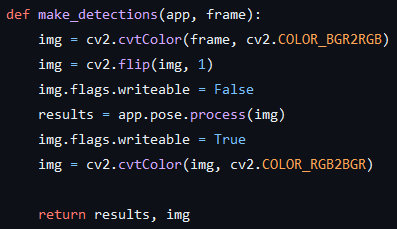
\includegraphics[width=0.49\textwidth]{figures/make_detections.png}
            \caption{Code Snippet of the make\_detections method in src/workouts/utils.py.}
            \label{fig:make_detections}
    \end{figure}
    
    The implementation of mediapipe detections can be seen in Figure \ref{fig:make_detections}. This snippet shows the raw camera input being preprocessed for the mediapipe pose processing, first the colour format is converted from BGR (openCV format) to RGB (mediapipe format), then flipped horizontally, and finally the frame's flags are set to be immutable. Once the processing of the frame is done, the flags are set to be once again mutable and the colour format is returned to BGR.

    The angle of the relevant joints to the exercise are calculated using the function seen in Figure \ref{fig:calculate_angle}. This function takes in three 2D points a, b, and c; and returns the angle between ab and cb in degrees.

    \begin{figure}[htbp]
            \centering
            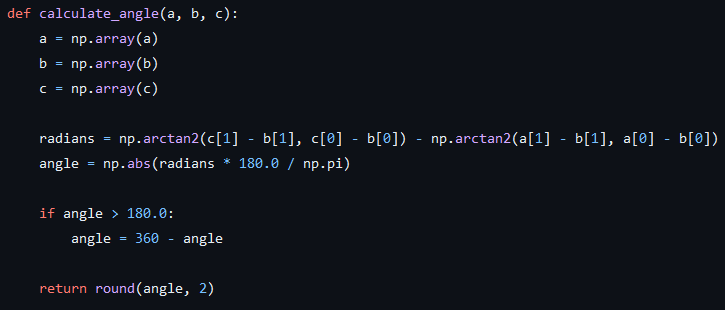
\includegraphics[width=1.00\textwidth]{figures/calculate_angle.png}
            \caption{Code Snippet of the calculate\_angle method in src/workouts/utils.py.}
            \label{fig:calculate_angle}
    \end{figure}

    Next is the repetition counting functionality which is shown in Figure \ref{fig:rep_counter}. This function is made to be generalise for it to be usable for every exercise type. It takes in as parameters the application that is using it, the current angle at the joint, the side (left or right), the low threshold the angle needs to reach for the repetition to count, the high threshold the angle needs to reach for the repetition to count, and the stage at which the muscle is at tension (or the stage that is harder to reach due to the mass of the weight). First it recovers the current count and the current rep stage, then it detects whether there has been a change in the rep stage. The rep stage will have changed from up to down if the current stage is up and the angle is above the high threshold and it will have changed from down to up if the current stage is down and the angle is below the low threshold. Then is updates the counter for the correct side.

    \begin{figure}[htbp]
            \centering
            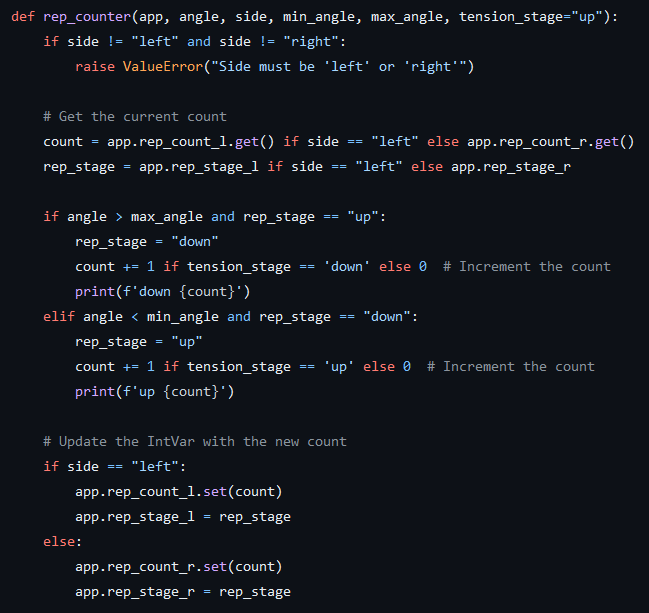
\includegraphics[width=0.75\textwidth]{figures/rep_counter.png}
            \caption{Code Snippet of the rep\_counter method in src/workouts/utils.py}
            \label{fig:rep_counter}
    \end{figure}
    
    Finally the culmination of these feature can be seen in Figure \ref{fig:detections}
    
    \begin{figure}[htbp]
            \centering
            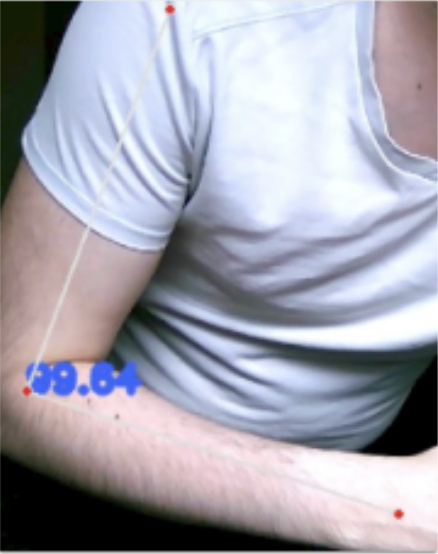
\includegraphics[width=0.34\textwidth]{figures/Screenshot 2024-08-18 at 19.07.46.png}
            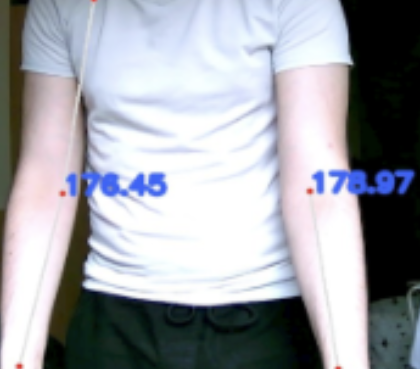
\includegraphics[width=0.49\textwidth]{figures/Screenshot 2024-08-18 at 19.08.36.png}
            \caption{Screenshots from the development of the bicep curl app. It shows mediapipe's keypoint detections on the arms and displays the angle between the shoulder-elbow segment and the wrist-elbow segment.}
            \label{fig:detections}
    \end{figure}
        
\section{GUI Creation}
    \subsection{Frontend Development}
        The frontend was developed using the tkinter library that is prepackaged into python. The GUI is organised like a tree system where each page is a node within the tree. To get to a page you must travel the GUI tree from the root node (home page) through the branches that lead to the desired page. Each branch can be traversed in both directions and the program can be exited a any moment.\\
        Here is a list of some of the pages:
        \begin{itemize}
            \item \textbf{home.py}\label{item:home}: the root node containing links to register, login, and login as guest. A screen capture of the home page can be seen below in Figure \ref{fig:home}
            \begin{figure}[htbp]
                    \centering
                    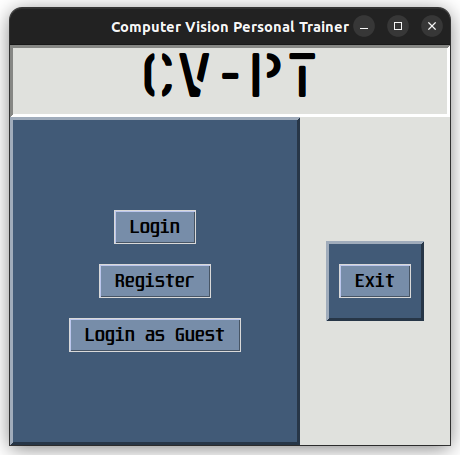
\includegraphics[width=0.49\textwidth]{figures/home.png}
                    \caption{Screen capture of the home page. (\ref{item:home})}
                    \label{fig:home}
            \end{figure}
            \item \textbf{register.py}\label{item:register}: contains a registration form that will save the users username and password to the database. If successful, it will send the user to menu.py.
            \item \textbf{login.py}\label{item:login}: contains a login form that checks if the username exists and the (hashed) password matches. If successful, it will send the user to menu.py. Screen captures of the login and register pages can be seen below in Figure \ref{fig:login_register}
            \begin{figure}[htbp]
                    \centering
                    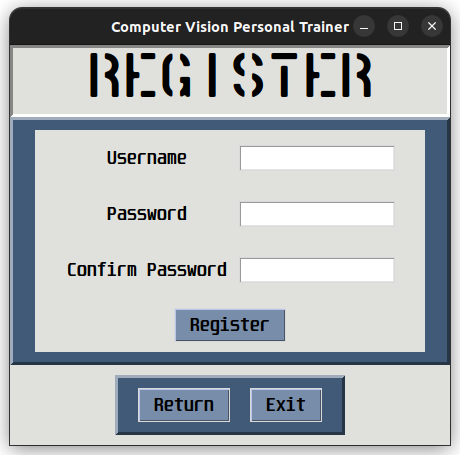
\includegraphics[width=0.49\textwidth]{figures/register.png}
                    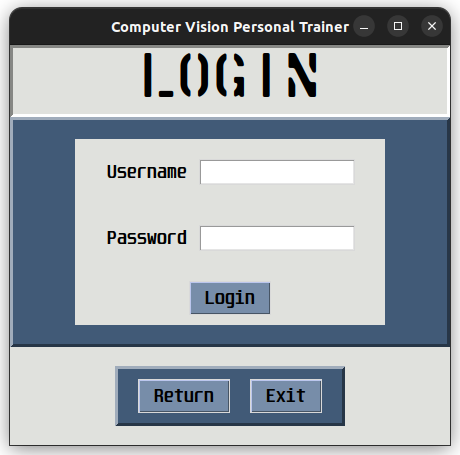
\includegraphics[width=0.49\textwidth]{figures/login.png}
                    \caption{Screen captures of the register (left \ref{item:register}) and login (right \ref{item:login}) pages.}
                    \label{fig:login_register}
            \end{figure}
            \item \textbf{menu.py}\label{item:menu}: contains a grid of buttons that link to each general muscle group/exercise type (arms, back, cardio, chest, legs, shoulders). If the user is logged in, there is also a button that links to the user's workout history. Screen captures of the menu pages with and without the history button can be seen below in Figure \ref{fig:menu}
            \begin{figure}[htbp]
                    \centering
                    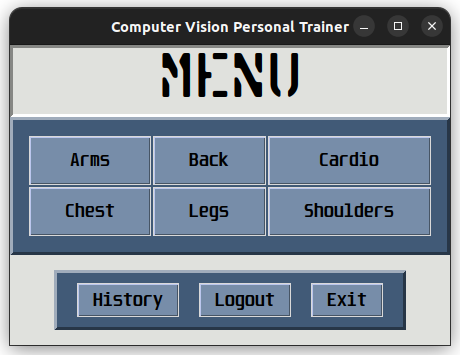
\includegraphics[width=0.49\textwidth]{figures/menu_with_login.png}
                    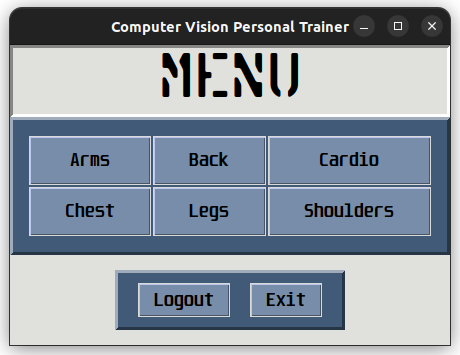
\includegraphics[width=0.49\textwidth]{figures/menu_without_login.png}
                    \caption{Screen captures of the menu page with (right) and without (left) a user logged in. (\ref{item:menu})}
                    \label{fig:menu}
            \end{figure}
            \item \textbf{arms.py}\label{item:arms}: contains a list of buttons linking to specific exercises (bicep curls and tricep pushdowns). The other child nodes of menu.py are the same where they are a list of the exercises relevant to that muscle group. A screen capture of the arms page can be seen below in Figure \ref{fig:arms}
            \begin{figure}[htbp]
                    \centering
                    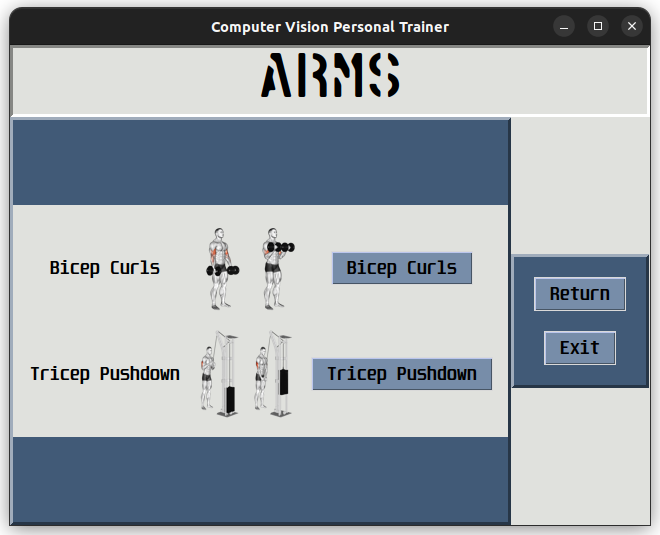
\includegraphics[width=0.49\textwidth]{figures/arms.png}
                    \caption{Screen capture of the arms page. (\ref{item:arms})}
                    \label{fig:arms}
            \end{figure}
            
            \item \textbf{bicep\_curls.py}\label{item:bicep}: These exercise pages are arranged to have a camera feed on the left half of the window and parameters and information on the right half. The camera feed will show the user what they are doing and act like the mirror in the gym, useful for visualising their form. Aswell as displaying the mediapipe skeleton on top of the joints that are relevant to the specific exercise. The right half has input areas where the user can enter the weight they are using, the amount of rest time they wish to have between sets, and depending on the exercise, which side of the body they are currently training. There is also a textbox that will display information at the top centre of the right half. A screen capture of the bicep curls app can be seen below in Figure \ref{fig:bicep}
            \begin{figure}[htbp]
                    \centering
                    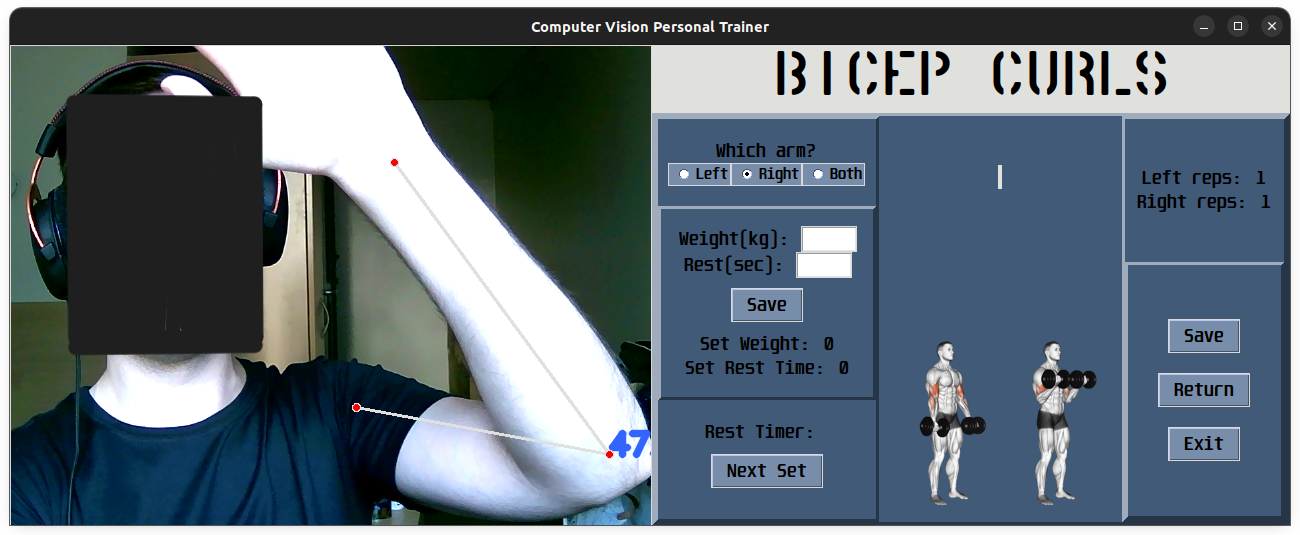
\includegraphics[width=0.99\textwidth]{figures/biceps.png}
                    \caption{Screen capture of the bicep curls page. (\ref{item:bicep})}
                    \label{fig:bicep}
            \end{figure}
        \end{itemize}

    Every time a user logs in or out, a popup appears asking them to rate their current mood on a scale of 1 to 10. This popup can be seen in Figure \ref{fig:mood}
    \begin{figure}[htbp]
            \centering
            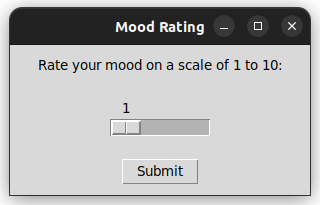
\includegraphics[width=0.49\textwidth]{figures/mood.png}
            \caption{Screen capture of the mood query popup. (\ref{item:bicep})}
            \label{fig:mood}
    \end{figure}
    
    \subsection{Backend Development}
        For the implementation of the backend I used the database management system called PostgreSQL. PostgreSQL is a relational database system written in the C programming initially released in 1996 that is free and open source. It functions also on Windows, MacOS, and Linux. As python language is also written in C, it has a strong library for database manipulation called pyscopg2.\\
        \subsubsection{Database tables}
            The schema contains three tables:
            \begin{enumerate}
                \item \textbf{users}:  (see Figure \ref{fig:users}) the users table contains five columns: 
                    \begin{itemize}
                        \item id (uuid, unique, primary key, not-null): unique identifier.
                        \item username (varchar, unique, not-null): unique username.
                        \item password (varchar, not-null): hashed password.
                        \item height (int): height of the user in centimeters, optional.
                        \item weight (int): weight of the user in kilograms, optional.
                    \end{itemize}
                    Each row refers to an individual user.
                    \begin{figure}[htbp]
                            \centering
                            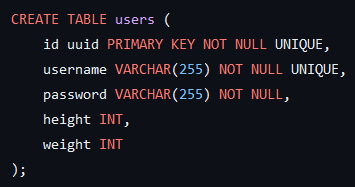
\includegraphics[width=0.67\textwidth]{figures/users.png}
                            \caption{Code Snippet of the SQL to create the users table}
                            \label{fig:users}
                    \end{figure}
                
                \item \textbf{sessions}:  (see Figure \ref{fig:sessions})the sessions table contains seven columns:
                    \begin{itemize}
                        \item id (uuid, unique, primary key, not-null): unique identifier.
                        \item username (varchar, foreign key, not-null): references the username of the user in the session.
                        \item created\_at (timestamp, not-null): timestamp at which the session started.
                        \item duration (interval): time interval between created\_at and the end of the session. Can be null because the row is created before the end of the session.
                        \item volume (int): the total weight moved by the user during the session.
                        \item start\_mood (int): the mood of the user at the start of the session on a scale of 1 to 10.
                        \item end\_mood (int): the mood of the user at the end of the session on a scale of 1 to 10.
                    \end{itemize}
                    Each row refers to an individual session.
                    \begin{figure}[htbp]
                            \centering
                            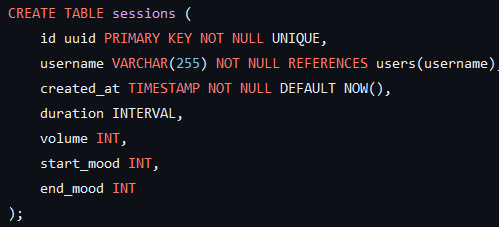
\includegraphics[width=0.67\textwidth]{figures/sessions.png}
                            \caption{Code Snippet of the SQL to create the users table}
                            \label{fig:sessions}
                    \end{figure}
                
                \item \textbf{workouts}:  (see Figure \ref{fig:workouts}) the workouts table contains eight columns:
                    \begin{itemize}
                        \item id (uuid, unique, primary key, not-null): unique identifier.
                        \item session\_id (uuid, foreign key, not-null): references the id of the session the workout belongs to.
                        \item name (varchar, not-null): the name of the excerce being performed by the user (e.g. bicep curls)
                        \item created\_at (timestamp, not-null): timestamp at which the workout started.
                        \item duration (interval): time interval between created\_at and the end of the workout. Can be null because the row is created before the end of the workout.
                        \item reps (int): number of repetitions the user performed during the workout.
                        \item max\_weight (int): the weight in kilograms lifted during the heaviest set during the workout.
                        \item volume (int): the sum of the number of reps times the weight of the set for each set performed during the workout.
                    \end{itemize}
                    Each row refers to an individual workout.
                    \begin{figure}[htbp]
                            \centering
                            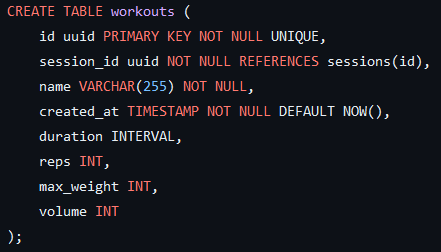
\includegraphics[width=0.67\textwidth]{figures/workouts.png}
                            \caption{Code Snippet of the SQL to create the workouts table}
                            \label{fig:users}
                    \end{figure}
                
            \end{enumerate}
            Another functionality that is provided by postgresql is the ability to create functions, also known as routines, to preform multiple SQL queries and actions.\\

        \subsubsection{Register functionality}
            The register system (see Figure \ref{fig:register} functions as follows: first there is a equality check between the password and the confirm password entries inputted by the user. If they match, then a connection to the database is made with DBConnection (see Figure \ref{fig:DBConnection}). 

            \begin{figure}[htbp]
                    \centering
                    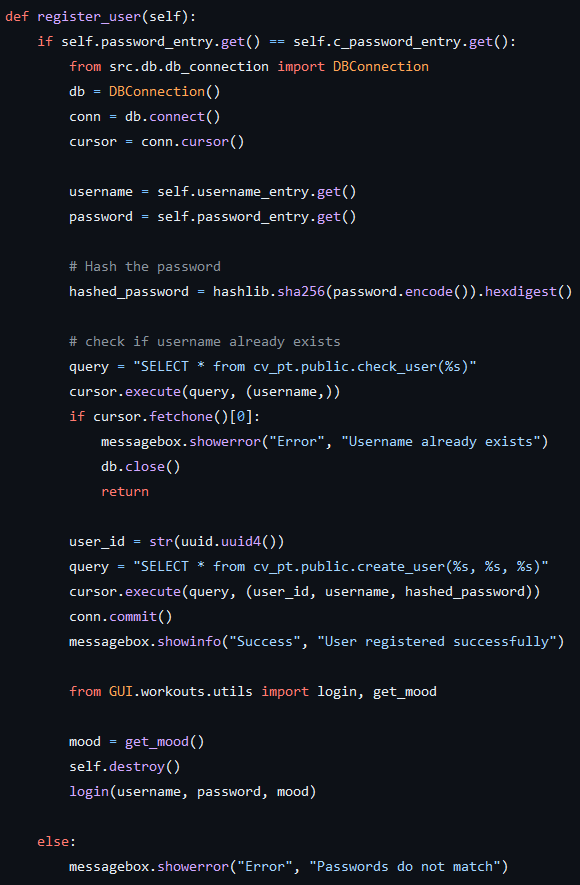
\includegraphics[width=0.9\textwidth]{figures/register_code.png}
                    \caption{Code Snippet of the register function}
                    \label{fig:register}
            \end{figure}

            Then, the password is hashed using the sha256 hashing function, and the users table is scanned for the username. If the username already exists, the process is stopped and the user is notified though a messagebox that their chosen username is already taken. Else, if the username is not taken, a new user is added to the users table with a universally unique identifier (uuid), the username, and the hashed password. The user is then automatically logged in (the login process is described next). 

        \subsubsection{Login functionality}
            The login system (see Figure \ref{fig:login_code}) functions as follows: first a connection to the database is formed using DBConnection (see Figure \ref{fig:DBConnection}).
            
            \begin{figure}[htbp]
                    \centering
                    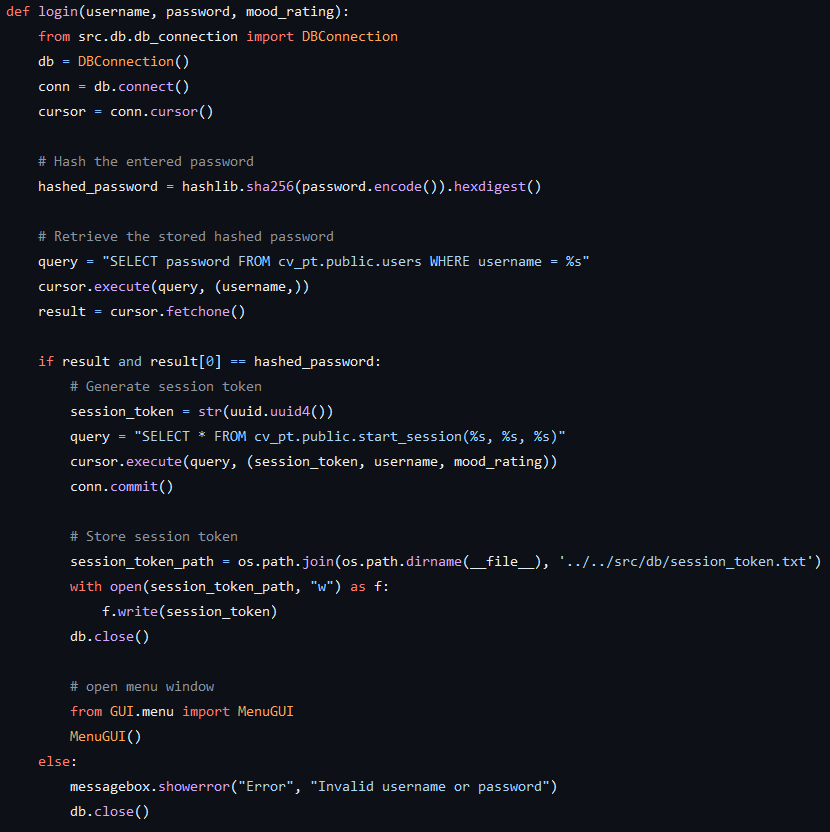
\includegraphics[width=0.99\textwidth]{figures/login_code.png}
                    \caption{Code Snippet of the login function}
                    \label{fig:login_code}
            \end{figure}

            Following that, the password entered by the user is hashed using the same hashing algorithm used for the encryption of the passwords and the database is searched for a user who has both matching username and hashed password. If a user is found, a new session is created, with a uuid which acts as the session token. This token is both stored in the database and also a newly created text file that only exists if a user is logged in.

            \begin{figure}[htbp]
                    \centering
                    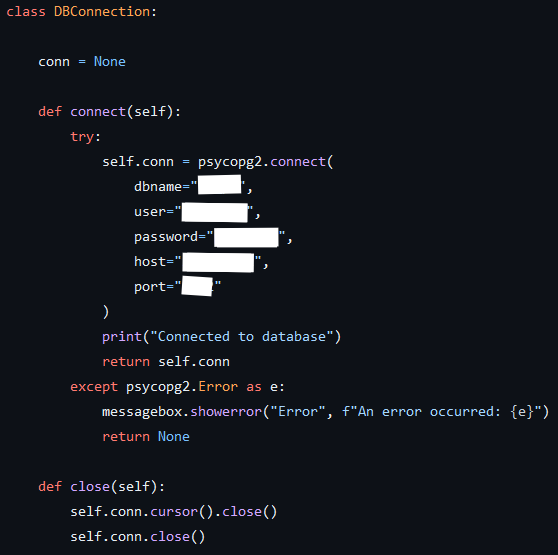
\includegraphics[width=0.67\textwidth]{figures/DBConnection.png}
                    \caption{Code Snippet of the DBConnection Class}
                    \label{fig:DBConnection}
            \end{figure}
            
            Finally, the menu GUI page is opened. If there are no matching users, a messagebox appears notifying the user that either the username or password is invalid and the connection to the database is closed. Which one of the username and password being invalid is not specified for security reasons, because if there is an indication that the username exists, it would be easier to brute force a login.\\  

            Figure \ref{fig:DBConnection} shows how to connect to a postgresql database using the psycopg2 library in python. 
        
    \section{Testing and Debugging}
    % Discuss the methods and tools used to test the system for functionality, performance, and reliability. Include the process of identifying and fixing bugs or issues.
    \subsection{Integration Testing}
        Testing whether the integration of the application into the GUI was fairly simple. All that needed to be done was to run the program and see if it displays. The first issue encountered was how to convert the default popup window openCV produces into a tkinter frame. This was solved by having the application be initialised as a tkinter frame by wrapping it in a class that inherits from ttk.Frame and running $super().\_\_init\_\_(parent)$ where $parent$ is a parameter of the application.\\
        The second issue was that the application would not open if an application had previously been opened during the program's uptime. This was caused by the application not closing properly when the window was closed. This was solved by creating a close method in the application class that destroys the application (see Figure \ref{fig:close}) and calling it when closing the window.
        
        \begin{figure}[htbp]
                \centering
                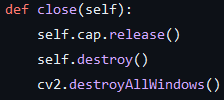
\includegraphics[width=0.49\textwidth]{figures/close.png}
                \caption{Code Snippet of the close method in src/workouts/arms/bicep\_curls.py}
                \label{fig:close}
        \end{figure}

    \subsection{System Testing}
        For the testing of the backend system, no major bugs where encountered as I have had previous experience with setting up a postgresql database in the past and had knowledge on how to avoid issues. I must also say that the integration of database management in PyCharm facilitated the task significatly.

% Results & Discussion
\chapter{Results \& Discussion}
% This section should present the findings of your work, and discuss them in the context of your original aims & objectives.  For software-oriented projects, how well does it meet your original requirements? Provide data where possible, e.g., results of user testing, performance measures, etc. For research-oriented projects, you should present the data in an appropriate format (tables, charts, visualisations) and provide a critical discussion around the results that provides insight and direction for future work.

%This chapter should present the results of your work, be they in the form of a software product, experimental research findings, or both. You should also link these results to your original objectives.

% goal ~2.5k words
% actual 1057 words

\section{Performance Evaluation}
    As there is no ground truth to compare the detections to, the evaluation of the detections will have to be qualitative rather than quantitative. That being said, the detections seemed to struggle when the lighting was too unfavorable such as when in a very sunny environment, and they also struggled to detect the user for the first time when their entire body wasn't visible, once a detection was made the users where able to get closer to the camera hiding parts of their bodies out of frame. The detections function both with the user facing the camera and with the user looking perpendicularly to the camera's line of sight. The accuracy of the angle calculation does seem to be lower when the user is facing the camera directly as the angle calculations do not currently use the z-axis (depth).\\
    When all the relevant joints were in frame, the repetition counting was very accurate when testing, but when one or more of the joints went out of frame, a large number of false positives were counted. This can be solved by instructing the user to step further away from the camera or change the angle of the camera so that all the joints are in frame.\\
    The performance of the database management system is sufficiently capable for the current scale and scope of the program, this will need to be revisited if the program reaches a much larger userbase.\\
    The performances of the GUI and user experience are described in section \ref{sec:feedback}
    
\section{Comparison with Existing Solutions}
    While some virtual coaching solutions already exist, such as the Apple Watch and Samsung Galaxy Watch, it would be interesting to compare existing virtual coaching against computer vision-based systems. Both of the wearables do great jobs at health and fitness tracking, from heart rate monitoring and ECG, through monitoring blood oxygen levels to sleep tracking. They offer real-time feedback during workouts, automatic workout detection, integration with third-party fitness apps, making them quite versatile tools for various types of exercises. These watches, however, are limited as they are unable to detect the exact position and pose of the user, making them less efficient at detecting poor form. They provide no visual feedback at all during the exercise; only auditory and haptic feedback. Moreover, they can only automatically detect exercises that involve arm movement. This is quite opposite to computer vision-based systems, which work best for movement analysis and real-time feedback on the form and technique of exercises. Such information cannot be provided with regular wrist-based wearables. While smartwatches may be portable and convenient, computer vision-based systems can be much more accurate and richer in the movement analysis, hence highly effective for detailed coaching and corrections in form. The primary feature that the watches are capable of that visual methods can't is heart rate monitoring of vital signs including the measuring of blood oxygen, body temperature, and sleeping patterns. In theory the wearables are well placed to judge arm movements, but due to the fact that they are only worn one a single wrist, the user is constrained to bilateral exercises or to move the wearable to the other wrist to perform unilateral sets. The watch being positioned on one side of the user also allows the user to have poor form on the side that is not tracked. One advantage that wearables have over computer vision based methods is that it is not prone to poor camera placement and angles which would limit the effectiveness of the detections and quality of the recommendations.
\section{User Feedback and Usability Testing \label{sec:feedback}}
    %get Mum, Dad, and Connie to test  
    The login and register are reported as easy to use and simple to understand, they are familiar because they are similar to the login/register commonly found on websites. The history page received very positive feedback, with the user stating that it provides a quick summary that will be good for future workouts to know at what weight to start at, avoiding having to do sets at weights that are potentially too low to be effective or so high that they risk injury. They also stated that they appreciated the two list format. There was also very positive comments on the instant visual feedback provided by the camera and the visible skeleton of the body parts in motion during the exercise.\\
    The main complaints came from the individual workout pages. There was confusion and annoyance with the rest timer, as the desired rest time would have to be re-entered after every set. The ease of understanding of the GUI was lacking, with no clear distinction between active time and rest time. The users expressed a desire for clearer instructions from the chatbox as at the time the only instruction was to set the rest timer if it had not already been done. The legibility at a distance of the text both on the camera side and the controls side was said to be poor, in particular  the repetition counter at the top right corner.\\
    Many recommendations were suggested and have been taken note of for improvement, such as moving the repetition counter to be on top of the camera feed and in larger font, adding more descriptive instructions to the chatbox, and having a "start set" button to make the application easier to understand.
\section{Limitations of the Project}
    Due to the very short time-frame in which this project needed to be planned, designed, programmed, and written up, the scope of this project was very restricted. As mentioned in previous sections of this report, there are many possible improvements that I would have liked to be able to implement but was not able due to lack of time. This includes having functionality for more than the two arm exercises that were implemented, having a more functional chatbox that would give feedback to the users specifically about their form, and not having the time to train, nor to obtain user feedback from more users. I also lacked the ethical approval for data collection for a deep learning model for repetition counting and form recommendations, which is something that would have greatly improved this project. As I am a single student developer and not a team of professional software engineers, this project was never going to result in a completed program with all the functionality required for public use, this is why this project acts more as a proof of concept and a foundation on which more research can based on. 

% Conclusion
\chapter{Conclusion}
% This is another relatively short chapter that is an opportunity to reflect on the project as a whole. Discuss the limitations and successes of the project, highlighting opportunities for future work. 

%This chapter should summarise the work you have undertaken by revisiting your project aims and objectives and what you have achieved to meet them. You should include a summarised response to any additional research questions you addressed. It is also important to discuss the limitations of the work and implications for future research in the space based on what you have done.

% goal ~200 words
% actual 363 words

\section{Summary of Project}
    This Project sought to create a computer-vision based training coach for computerised physical training, by creating a computer program capable of making recommendations on physical exercises and form to its users based on camera input where the users' body and movements are detectable.
    Implementing this project involved the creation of an application that is capable of the aforementioned tasks and embedding it into a graphical user interface that is easy to navigate and provides the necessary information to the user. A simple backend was attached allowing for a login system with workout history and mood tracking.
    
\section{Contributions to the Field}
    This project contributed to the field of both computer science and more specifically human pose estimation but also to the fields of sports psychology and physical training. By creating this program, many research avenues have been facilitated and opened up in terms of studying the effect of exercise on mood and mental health and on how computer vision, HPE, and robotics in general can help in this sector.   
    
\section{Practical Implications}
    This project acts as a baseline from which further research can be make. Allowing for experts and researchers in the field of sports and physical health to utilise computer vision technologies to perform studies on not only the impact of exercise on mood and mental health but also many more questions. This program, if improved and iterated upon, could have profound positive implications on public health in terms of getting the general population to exercise more and improve our understanding of certain workouts and how they are performed optimally.
    
\section{Recommendations for Future Work}
    There is still much more that can be added to this program. More types of exercises, better recommendation system, using deep learning methods to train a recommendation model, and much more in terms of the application. Another recommendation for future work would be to port the program as a smartphone application, this will obviously require work on server side implementations and allowing models to either be much smaller while keeping their accuracy or be able to run on cloud computing.
\section{Final Thoughts}
    Overall, even though I would have liked to have been able to implement more functionality into my application, I believe that this have laid a good foundation for future research.



% end of thesis body
% --------------------------

% Print out the references
\printReferences


\end{document}
